\documentclass[12pt,letterpaper]{article}
\usepackage{times}
\usepackage[utf8]{inputenc}
\usepackage[spanish]{babel}
\usepackage[authoryear]{natbib}
\usepackage{amsthm,amsmath,amsfonts,amssymb}
\usepackage[doublespacing]{setspace}
\usepackage{graphicx}
\usepackage{tabularx}
\usepackage{caption}
\usepackage{subcaption}
\usepackage{arydshln}
\usepackage{lscape}
\usepackage{pdflscape}
\usepackage{hyperref}
\usepackage{cleveref}
\usepackage[top=3cm, bottom=3cm, left=3cm, right=3cm]{geometry}


%\usepackage{setspace}
%\singlespacing
%\onehalfspacing
%\doublespacing
%\setstretch{1.1}

\title{Tipo de Cambio Real de Equilibrio de Bolivia} 

\author{Hugo Pablo Rocha Portugal \and Paola Cecilia Yujra Tonconi}
%\author{10195}

\date{14 de septiembre de 2018}

\begin{document} 

\maketitle 

\begin{abstract}
\singlespacing

En el presente documento está contextualizado alrededor de la discusión del paradigma de crecimiento económico basado en la competitividad externa. Para contrastar esta idea, se analizan las políticas cambiarias bolivianas que buscaron este objetivo. Para dicho efecto, se plantea estudiar el desempeño de las mismas con respecto a la senda de equilibrio del tipo de cambio real. El análisis permite no solo determinar la relevancia y compatibilidad de estos métodos con las características particulares de la economía revisada, sino también propone elementos importantes para poder construir una medida más relevante y apropiada de equilibrio. En el documento se encuentra que el tipo de cambio real no es una medida de competitividad externa para las exportaciones bolivianas aunque tienen un efecto particular en las importaciones. Por otro lado, se propone que la política cambiaria de tipo de cambio nominal no es la mejor manera de estimular cambios en el TCR. Finalmente, se encuentra el conjunto de fundamentos relacionados con la dinámica de la serie en cuestión.
\\
\\
\bigskip
Palabras clave: Estimación, BEER, DEER, Tipo de Cambio Real, Economía abierta \\
Clasificación JEL: E500, F140, C510

\end{abstract}

\newpage

\section{Introducción}

Tras la devastadora hiperinflación que Bolivia sufrió durante la primera mitad de la década de los ochenta, la economía boliviana se restituyó habiéndose logrado una solución satisfactoria que puso fin a dicha patología en precios poniéndole un alto a la depreciación descontrolada de la moneda mediante la unificación de los mercados cambiarios y la instauración de una nueva moneda: el boliviano. Sin embargo, características como el contrabando, la informalidad, la corrupción, la pobreza y la dolarización se fueron agudizando en la economía durante el posterior periodo de estabilización. La precaria situación económica estaba determinada por un proceso de insipiente crecimiento debido al enfoque extractivo primario y al comercio informal que crecía. Estos elementos determinaron la dependencia a las importaciones, y la política económica referente de la época fue el establecimiento del régimen cambiario \emph{crawling peg} orientado a las mini-devaluaciones. 

La sostenida devaluación de la nueva moneda local generó una alta dependencia al dólar americano y limitó la efectividad de la política monetaria. Los precios en bolivianos de los bienes importados subían constantemente por el costo elevado de importación determinado por la constante depreciación de la moneda local, haciendo que la preferencia por moneda se traslade a la divisa estadounidense. En otras palabras, las expectativas de la población con respecto al tipo de cambio boliviano estaban ancladas en la depreciación y los agentes económicos respondían a la perdida del poder adquisitivo de la moneda local utilizando el dólar americano para compra de bienes importados y ahorro. Al mismo tiempo, no existía la suficiente producción interna para cubrir la demanda interna y así sustituir las importaciones. Este hecho combinado con los bajos niveles de remuneración y precariedad del mercado laboral segmentado y discriminatorio profundizaron la informalidad y el contrabando. Ambas características están inter-relacionadas entre ellas y determinarían una alternativa laboral flexible y, al mismo tiempo, una forma barata de satisfacer la demanda de bienes de la población.

Al mismo tiempo, las condiciones particulares por las que la economía pasaba no permitieron cambiar de matriz productiva al paradigma industrial, a diferencia de los vecinos regionales que ya habían logrado realizar la transición décadas atrás; la explotación de materias primas para exportación aún constituía el paradigma de crecimiento de la economía boliviana, así como lo fue desde épocas coloniales y durante toda la república. Por un lado, los elevados costos de capital importado de producción limitaron la llegada de nuevas tecnologías estacando al sistema productivo en procesos precarios caros y de intensiva participación de la mano de obra. Este hecho generó que la búsqueda de competitividad en precios se realice a través de la reducción de costos sacrificando productividad y calidad mediante la baja remuneración a los factores productivos, en un esquema de debilidad institucional que no velaba por el bienestar económico del trabajador. Como consecuencia de ello, el crecimiento económico en la década de los noventa se procuró el cambio de esquema económico productivo con la capitalización de algunas empresas estatales, lo cual generó resultados limitados durante este proceso de recuperación económica mientras se gestaba una clima de inestabilidad política. Sin embargo, a mediados de la década de 2000's, la mayor incursión de los hidrocarburos bolivianos en mercados internacionales y el incremento de precios de materias primas constituyen los elementos claves para que Bolivia presente mejorías en sus indicadores macroeconómicos y sociales bajo la estructura extractivista que caracteriza a su economía.

%Exito económico
El éxito del país en materia económica es sobresaliente desde 2004-2005 hasta 2014. Efectivamente, el país pasó de ser uno de los más pobres del subcontinente a tener el crecimiento económico más importante de la región. Al mismo tiempo, consiguió recaudar elevados niveles de Reservas Internacionales Netas (RIN), reducir los niveles de pobreza y desigualdad, des-dolarizar su economía, reducir los niveles de deuda y mantener niveles controlados de inflación. Incluso cuando los términos de intercambio no le favorecieron, a partir de 2014, Bolivia demostró una gran capacidad de resiliencia aplicando políticas macro prudenciales y contra-cíclicas. Ante todos estos logros queda preguntarse cuales fueron los factores de política económica más importantes que contribuyeron a su consecución.

%Sector externo
Sin lugar a dudas, el desempeño de la balanza comercial en el periodo de expansión, destacado previamente, se constituye en el influjo de divisas y riqueza más importante desde finales de la década de los setenta. A partir de 2004 y consolidándose a finales de 2005, las exportaciones de hidrocarburos presentaron valores elevados los cuales se incrementaron significativamente periodo tras periodo. La nacionalización de 2006 fue una de las políticas nacionales más importantes pues permitió que el país capte, utilice y distribuya estas ganancias siendo que previo a esta medida quien se quedaba con la mayoría de las utilidades eran las empresas trans-nacionales que operaban la exploración y explotación de recursos naturales en Bolivia. Por estas razones, este fenómeno está altamente correlacionado con el citado éxito económico pues permitió a su vez que ocurra un shock positivo a los ingresos de la población. En este sentido, no es casualidad que la meta de las pasadas autoridades políticas y económicas del país haya estado orientada a procurar la bonanza de comercio internacional basando sus esperanzas en políticas dirigidas al desempeño del sector extractivo exportador.

En este periodo de boom, los impuestos directos a los hidrocarburos permitieron al gobierno, especialmente el central, incrementar su tamaño y emprender políticas públicas importantes como la implementación de bonos sociales dirigidos principalmente a niños, madres en gestación y adultos mayores, los cuales constituyen la población más vulnerable del país. Asimismo, dichos influjos derivados de la venta de hidrocarburos permitieron el incremento de las RIN y gasto e inversión pública ejecutados a través del gobierno central así como por los gobiernos departamentales y municipales. Los proyectos públicos con mayor notoriedad financiados por estos recursos fueron las Empresas Públicas Nacionales Estratégicas (EPNEs), obras en la red nacional de caminos y la construcción de infraestructura diversa. Al mismo tiempo, esta inyección de circulante en la economía, primero a través del gasto público, incentivó el gasto e inversión privados. En segundo lugar, después de 2014 aún se inyectan recursos en la economía a través de la política fiscal y monetaria con connotación contracíclica colocando dinero en el sistema financiero para fomentar el gasto privado especialmente a través del crédito para la vivienda social y el sector productivo. 

Acerca del tema de políticas cambiarias y monetarias se puede destacar que después del periodo de estabilización, la subida de precios internacionales de materias primas a partir de 2004-2005 trajo consigo, además del éxito exportador, un componente inflacionario importado el cual pudo ser contenido gracias al respaldo y confianza de la población en las RIN recién acumuladas. La política cambiaria de continuas depreciaciones que se llevaban a cabo hasta entonces cambió de dirección hacia la apreciación del boliviano y una política monetaria contractiva. Estas medidas contribuyeron, junto a otras, a la des-dolarización financiera de la economía. Habiéndose contenido las presiones inflacionarias, la crisis financiera internacional 2008-2009 generó la demanda de dólares en la economía generando presiones de devaluación que fueron contenidas con la estabilidad cambiaria. Tras este evento, el repunte de los precios internacionales y otras crisis externas durante 2010-2011 implicaron la reaparición de presiones inflacionarias que fueron combatidas apreciando la moneda por un último periodo. Finalmente, a partir de 2012 se ha estabilizado el movimiento cambiario hasta la actualidad sin mayores presiones inflacionarias externas. En resumen, el Banco Central de Bolivia (BCB) aduce que la estabilidad cambiaria actual ha permitido mitigar las presiones inflacionarias de origen externo, anclar las expectativas de los agentes económicos con respecto del valor del dólar y des-dolarizar financieramente la economía. Sin embargo, después de la caída de precios internacionales en 2014, el BCB, a pesar de mantener invariante su política cambiaria, cambió su postura monetaria debido a la desaceleración que este shock externo implicó. Por ende, se consolidó una perspectiva anti-cíclica de la orientación de la política monetaria inyectando recursos en la economía a través del sistema financiero.

En contraste y para dar contexto a la política cambiaria en la etapa de boom, durante la década de los noventa y tras la estabilización post-hiperinflación, el crecimiento económico a través de exportaciones, la des-dolarización, la ejecución soberana de la política monetaria se constituyen en el santo grial perseguido por los hacedores de política bolivianos que a través de la devaluación cambiaria procuraron generar la suficiente competencia externa para lograr dicho cometido. Es decir, plantearon a la devaluación nominal como el instrumento para devaluar el tipo de cambio real (TCR) en la dirección que permita incrementar las exportaciones. Esto debido al paradigma económico, que se manejó e incluso aún se maneja, basado en que la competitividad de tipo de cambio fomentaría las exportaciones de recursos naturales constituidos en materias primas y estos a su vez generarían utilidad económica y entrada de divisas, activos con los cuales se conseguiría la solución a todos los problemas inmediatos y acumulados de la economía nacional los cuales son reclamos de la sociedad boliviana. Bajo este concepto, es importante estudiar el periodo de apreciaciones nominales que permitió la consecución de los objetivos buscados con competitividad externa y éxito comercial internacional en la década de los 2000's y 2010's.

%TCR como nivel de competitividad
Debido a la importancia que las exportaciones tienen para la economía de Bolivia es pertinente estudiar aquellas variables económicas que las fomentan y los comovimientos que comparten. Si bien los términos de intercambio y la nacionalización de hidrocarburos, sin lugar a duda, beneficiaron al crecimiento interno del país, se deben identificar las políticas económicas que hayan logrado o podido haber logrado aprovechar el importante periodo de bonanza. En este contexto, la más importante de ellas es la política cambiaria que podría haber definido el tipo de cambio real que teóricamente captura la competitividad de los productos bolivianos comparado con sus principales socios comerciales. Teóricamente, la depreciación de esta variable implicaría el abaratamiento de los bienes y servicios nacionales haciéndolos más atractivos para sus compradores internacionales, generando el incremento de las exportaciones.

%TCReq para saber cual es la mejor política cambiaria, cuanto cuesta mantener el tipo de cambio fijo y desalineamientos y como se mueve
En este marco, se propone estudiar el tipo de cambio real desde la perspectiva de su equilibrio. Esto permitiría encontrar el nivel de balance entre el denominado equilibrio interno y externo, es decir, el tipo de cambio real que propiciaría la competitividad externa y condiciones internas de la economía para lograr crecimiento sostenible. Los valores observados del TCR y su variable calculada de equilibrio determinan el desalineamiento cambiario al que se puede atribuir los déficits en balanza comercial y se constituirían en condiciones que limitarían el crecimiento de la economía interna. Al mismo tiempo, el análisis podría indicar cual es la mejor política que se podría haber aplicado y se puede aplicar en el futuro. Adicionalmente, la estimación de este equilibrio cambiario, otorgaría información sobre el set de variables que llegan a determinarlo a través de la política económica.

%Lo que se encuentra en el paper
En este sentido, se utilizan dos metodologías convencionales y complementarias para calcular el tipo de cambio real de equilibrio, las cuales son \emph{behavioral equilibrium exchange rate} BEER y \emph{desired equilibrium exchange rate} DEER. La primera aproximación se enfoca en establecer los determinantes que se espera tengan efectos persistentes y de corto plazo en el TCR. Esta metodología encuentra que el TCR en tendencia siempre se mantiene bajo la senda de su equilibrio con leves desviaciones de corto plazo del mismo, el objetivo de esta metodología es encontrar los movimientos de los fundamentos que minimizan dichas desviaciones. La segunda metodología propone que los desalineamientos se encuentran antes de 2006 y después de 2014, momentos en los que los precios en materias primas no beneficiaron los términos de intercambio. El uso complementario de estas dos metodologías permiten entender, a través del primer modelo, cuales son las variables que afectan el movimiento del TCR y su correspondiente equilibrio y, mediante el segundo modelo, se puede observar cuál es el nivel de depreciación del tipo de cambio real que mejora los niveles de cuenta corriente. Sin embargo, a partir de un análisis más profundo, se encuentran debilidades en el uso de estas metodologías que son utilizados como focos de estudio que permiten entender mejor la economía boliviana y sus particularidad a través de las cuales se puede reconsiderar una mejor forma de medir el tipo de cambio real de equilibrio.

Este documento encuentra que la variable que explica los incrementos de exportaciones e importaciones son las demandas externas e internas respectivamente. Por otro lado, el tipo de cambio real es una medida adecuada de competitividad para las importaciones de bienes finales, su apreciación se puede entender como un factor que, junto al crecimiento económico del país, podría haber ayudado a fomentarlas sin perjudicar los elevados valores de exportaciones, sin embargo, el efecto ingreso prima al efecto que pueda haber tenido el TCR en el comportamiento de ambas series. A pesar de esta última consideración, se identifica una baja sensibilidad de las importaciones frente el TCR potencialmente debida a la baja capacidad nacional de sustitución de importaciones. Esta insensibilidad del TCR se repite para el caso de las exportaciones. En este sentido, el tipo de cambio real no es una medida cabal para entender la competitividad externa en el contexto boliviano pero si parece medir una parte pequeña del poder de compra de la moneda boliviana. 

Además el presente estudio propone por primera vez una identificación estructural de equilibrio parcial de fundamentos del tipo de cambio, la cual si bien no es nueva en la literatura internacional, no ha sido revisada empíricamente para el caso boliviano. Al mismo tiempo, se propone un conjunto de proxys para dicha operativización. En este sentido, las variables que parecen influenciar en el corto plazo al TCR son el ratio de proxys de productividad nacional con respecto al de los socios comerciales bolivianos, el gasto de gobierno en no transables, los términos de intercambio y los activos externos netos. Los resultados indican una débil posibilidad de afectar mediante la política económica a los desequilibrios de corto plazo del TCR.

Bajo esta motivación el presente documento plantea la consideración de elementos importantes del tipo de cambio real y de la medición de su equilibrio en la sección \ref{pre}; posteriormente, se define la metodología a ser utilizada en la sección \ref{tcr}; la verificación de series estadísticas, hechos estilizados y resultados son planteados en la sección \ref{calc}; se continúa con la reflexión de los resultados encontrados en la sección \ref{consid} y para sintetizar lo estudiado, la sección \ref{concl} concluye el documento.

\section{Revisión de Literatura}\label{pre}

\subsection*{Tipo de cambio real}
%TCR
El tipo de cambio real es la variable que refleja cuánto de una canasta básica doméstica es necesaria para comprar una canasta básica extranjera. Esta variable es determinada por la siguiente relación:
\begin{equation}\label{tcr1}
Q_t=E_t\frac{P_t^*}{P_t},
\end{equation}
donde $Q_t$ es el tipo de cambio real, $E_t$ es el tipo de cambio nominal, $P_t^*$ representa el índice de precios de una canasta básica representativa de una economía extranjera y $P_t$ es el índice de precios de una canasta básica doméstica representativa. En logaritmos la expresión \ref{tcr1} es representada por:
\begin{equation}\label{tcrlog}
q_t=e_t+p_t^*-p_t.
\end{equation}
Nótese que las minúsculas describen a la variable en logaritmo. Tanto las expresiones \ref{tcr1} y \ref{tcrlog} representan el poder de compra de una moneda frente a otra. El tipo de cambio real también puede ser analizado en términos de precios transables y no transables. Para tal efecto, en el caso de la ecuación \ref{tcrlog} se asume que $p_t=\alpha p_{Nt} + (1-\alpha)p_{Tt}$, donde $0<\alpha<1$, $\alpha=\alpha^*$, en este contexto, $p_{Nt}$ es el precio de no transables, $p_{Tt}$ el de transables y $\alpha$ es la proporción de precios de bienes no transables que constituyen el índice de precios. Entonces:
\begin{equation}\label{tcr2}
q_t=q_{Tt}+\alpha(\hat{p}_{Nt}-\hat{p}_{Tt}),
\end{equation}
donde, el circunflexo implica la diferencia de la variable entre precios domésticos y extranjeros, por ejemplo $\hat{p}_{Nt}=p_{Nt}^*-p_{Nt}$, y $q_{Tt}$ es el tipo de cambio real de bienes transables donde $q_{Tt}=e_t+p_{Tt}^*-p_{Tt}$. Por lo general, se asume que $q_{Tt}=0$ (o $Q_{Tt}=1$) debido a que los precios transables, por el concepto de competitividad y bajo los mismos supuestos de competencia perfecta, tendrían el mismo valor tanto en la economía doméstica como en el exterior comparados en una misma moneda. 

Las ecuaciones \ref{tcr1} y \ref{tcrlog} son análogas e implican que, manteniendo todo lo demás constante, los incrementos de tipo de cambio nominal (devaluación nominal) o de los precios extranjeros o las caídas del nivel de precios local determinan una depreciación real de la moneda nacional. Lo contrario aplica para el caso de una apreciación real. Sin embargo, desde la perspectiva caracterizada en la ecuación \ref{tcr2}, el tipo de cambio real de bienes transables y la diferencia del nivel de precios no transables, y transables, entre el resto del mundo y la economía local determinan los movimientos del TCR. 

La ecuación \ref{tcr2} implica una perspectiva más analítica para estudiar la influencia de las políticas económicas sobre el TCR a través del efecto que generan en cada grupo de precios. Por ejemplo, el caso más estudiado entiende que el gasto público (política fiscal) se ejecuta sobre la compra de bienes no transables. Este shock de demanda sobre en el mercado de bienes no transables hace que los precios de estos se incrementen. 

Por otro lado, la teoría contemporánea no describe cual es el efecto de las otras políticas económicas sobre cada conjunto de bienes. Sin embargo, a continuación se ensayan algunas consideraciones al respecto. El impulso de la política monetaria (sin tomar en cuenta los efectos asimétricos sobre el nivel de precios) afecta a precios transables perecederos y no transables, como servicios y bienes locales cuyos precios dependen del dinamismo de la economía nacional y la inflación de transables. Estos últimos son determinados en mayor medida por los mercados internacionales teniendo en cuenta que pueden ser comprados y vendidos en el mercado internacional y tienen competencia internacional. Para que no haya arbitraje, los precios se ajustan a un equilibrio que rige a través de todos los países tomando en cuenta los costos y barreras de importación y exportación de cada economía y la calidad y características especiales de cada producto tiene, lo cual genera discriminación vertical en sus precios. 

Asimismo, la política cambiaria o el movimiento de las paridades de moneda tienen efecto en los bienes transables debido a que la depreciación (apreciación) encarece (abarata) el valor del bien en moneda local. Nótese que en este caso, los países afrontan un amplio nivel de exogeneidad en el sentido que la apreciación de la moneda de un país extranjero, del cual se importan bienes, implicará la depreciación implícita de la moneda local. Finalmente, se debe considerar el efecto que las políticas sociales, comerciales, financieras y laborales tienen sobre la competitividad de los precios finales de los bienes transables a través de la modificación de los costos de producción y su análisis es más complejo. 

Es importante destacar que la teoría económica moderna entiende que la política económica no tiene influencia en el cambio de tendencia del equilibrio de largo plazo del tipo de cambio real. Esto porque, dados los niveles de los fundamentos, la tendencia y el equilibrio estarían dados por la propia estructura de cada economía particular. En contraposición, el papel de la política económica está orientada en influir en los fundamentos para que el tipo de cambio real retorne a su nivel de equilibrio cuando se encuentre desequilibrado. Esta perspectiva implica que el TCR no puede estar desviado del nivel de equilibrio por mucho tiempo. Sobre como influir en el movimiento del tipo de cambio real se ampliará la discusión en la sección \ref{consid}.

Entonces, como se ha anotado previamente, las representaciones del tipo de cambio real de las ecuaciones \ref{tcrlog} y \ref{tcr2} son importantes por distintas razones. La primera, que está basada en el propio concepto de la variable, es utilizada para construir estadísticamente el indicador pertinente que caracteriza dicha variable. Por otro lado, la segunda expresión permite realizar una interpretación sobre las fuerzas que podrían influir en sus movimientos.

En este sentido, hay algunas consideraciones prácticas al respecto del tipo de cambio real que deben ser apuntadas. En particular, $p_t^*$ y $p_t$ no siempre representan precios de las mismas canastas básicas, esto porque distintos países consumen distintos bienes básicos, o en otras palabras, no todas las economías incluyen exactamente los mismos productos en sus canastas. Adicionalmente, esto se puede deber a que frente la modernización y aparición de nuevos bienes, los institutos de estadística tardan en actualizar sus listas de productos considerados en la canasta básica. En teoría, esto podría ocasionar algún ruido en el cálculo del tipo de cambio real que en promedio puede asumirse insignificante, aunque queda la duda hasta qué punto esto es perjudicial cuando una convergencia tarda en suceder.\footnote{Por ejemplo, ¿es relevante entre 2010-2017 incluir los servicios de telefonía pública (cabinas fijas y ambulantes), videoreproductor, VHS, minicomponente, walkman, discman y tantos otros dentro de la canasta básica?} Por otro lado, cuando se relaciona al TCR con el comercio internacional de, por ejemplo, materias primas, parece que esta medida cambiaria no tiene incumbencia pues, como ha sido expuesto, mide la relación de bienes que entran dentro de la canasta básica, a la cual las materias primas y demás insumos productivos son ajenos pero altamente comercializados internacionalmente. Finalmente, a pesar que algunos investigadores asumen que $q_{Tt}=0$, debido al supuesto de perfecta sustitubilidad de bienes transables homogéneos en competencia perfecta internacional de bienes transables, en este documento se considera importante tomar en cuenta la diferenciabilidad horizontal y vertical de bienes transables por lo menos al momento de realizar consideraciones derivadas de los resultados.

\subsection*{Tipo de cambio real de equilibrio}

Dada la definición del tipo de cambio real es preciso establecer la definición de su correspondiente equilibrio. El mismo es una variable no observada que idealmente podría ser considerada como el contrafactual positivo\footnote{Desde la perspectiva deontológica de la ciencia.} del tipo de cambio real. En otras palabras, es la variable que captura los valores ideales o en equilibrio de los componentes que conforman el TCR. En este sentido, se entiende como valor de equilibrio al tipo de cambio real que representa a la economía abierta que está en equilibrio tanto a nivel interno como externo. Las implicaciones de estar en equilibrio son discutibles porque implica distintas interpretaciones dependiendo de la perspectiva del autor.

El propio hecho que una variable denominada tipo de cambio real de equilibrio exista, indica que la ciencia social acepta tanto teórica como empíricamente que el tipo de cambio observado no corresponde a los valores de equilibrio de los mercados que lo definen. En este sentido, se entiende que existen distorsiones (transitorias o inesperadas) en dichos mercados que generan valores observados que podrían no corresponder a lo que deberían representar y en el peor de los casos retroalimentarse debido a algún tipo de persistencia. Estos pueden ser interpretados como las rigideces de precios. El hecho de reconocer esto implica asumir una postura teórica para identificar las distorsiones transitorias o no anticipadas. A su vez esto determinará el tipo de equilibrio que se considere y el consecuente método para calcularlo.

%Eq CP MP LP
Bajo esta premisa, \cite{driver2005concepts} distingue tres tipos de conceptos centrales de equilibrio utilizados y operativizados por distintos autores. Los de corto plazo que capturan movimientos de la serie correspondientes a los de sus fundamentos y a factores transitorios abstrayendo únicamente los shocks inesperados. Los de mediano plazo que se caracterizan por su compatibilidad con el balance externo e interno de la economía, es decir, esta perspectiva es consistente con los fundamentos en su nivel de tendencia, los mismos que pueden estar aún convergiendo, o no, a sus valores de estabilidad de largo plazo. Y, finalmente, el equilibrio de largo plazo que ocurre en pleno empleo y es compatible con los co-movimientos de los valores de largo plazo de sus fundamentos, en otras palabras, cuando no hay cambio endógeno de tendencia.

El concepto de equilibrio de corto plazo implica que los mercados están en equilibrio pero son afectados por impulsos transitorios y shocks inesperados. La remoción de estos últimos elementos constituye el objetivo operativo de estos modelos para encontrar el equilibrio. El concepto de mediano plazo, asume que los datos observados podrían no corresponder al equilibrio en los mercados que los generan; para contrastar esta hipótesis se encuentra la diferencia entre los niveles asumidos de equilibrio del sector interno y externo y los compara con los niveles tendenciales de las variables observadas. Finalmente, el concepto de largo plazo implica que para obtener el nivel de equilibrio del TCR todos los mercados y las correspondientes variables deberían estar en pleno empleo, entonces, a partir de los datos observados se construye una estructura de la economía que aproxima las interelaciones de las variables capaces de reproducir la conducta de la economía para entonces generar los valores de equilibrio abstrayendo los shocks inherentes de las series observadas.

%Eq interno externo
Entonces, asumir que el mercado interno y externo están siempre en equilibrio, y los datos observados son una reproducción de dicha relación, implica asumir un supuesto importante para determinar el concepto de equilibrio que vaya a ser ejercitado. En tal sentido, se propone utilizar ambas nociones, una que asuma que los mercados efectivamente están siempre en equilibrio aunque con las correspondientes rigideces de precios que afectan en el corto plazo y otra que asuma la existencia de un equilibrio más allá de lo observado. Sin embargo, antes de discutir estas perspectivas a profundidad se plantea revisar algunos matices de las características de los conceptos.

Con respecto a la perspectiva de largo plazo en la que los valores que se deben utilizar para encontrar la senda de equilibrio son los de \emph{steady-state} y pleno empleo, se debe establecer las siguientes consideraciones. Dichos resultados idealizados son obtenidos con base en valores pasados de las variables de la economía que determianrían el crecimiento vegetativo de una economía en particular. Esto implica pensar que la población crecerá a una tasa constante siendo que los factores de producción estarían siempre empleados y en equilibrio mientras todas las decisiones económicas en el sistema convergerían a través de la repetición sin cambios en la estructura que reproduciría dicha situación. 

Esto implica conocer la estructura del proceso generador de datos de la economía en particular. Se debe convenir que una economía y sus realizaciones no son simplemente el hecho de interacciones simplificadas de sus agentes, sino que cambios y diferentes direcciones son determinadas en la complejidad y heterogeneidad de los sistemas que la componen. Asimismo, se debe reconocer que los ámbitos políticos, culturales y sociales también tienen una influencia importante en el área económica. Todo esto sin tomar en cuenta los shocks exógenos e inesperados que puedan suceder.

En tal sentido, el trabajo de identificación de los sistemas macroeconómicos ha avanzado bastante en el contexto de países desarrollados. En estos últimos, las relaciones económicas productivas ya están consolidadas en sus mercados internos y en los mercados internacionales habiéndoles concedido la sostenibilidad de su desarrollo, lo cual facilita y hace más creíble el supuesto de convergencia a largo plazo. Esto debido a que su mejor alternativa es continuar replicando la fórmula explotando el aspecto de su economía en el que son más competitivos que el resto de los países y con el que les va bien internamente. 

En países en desarrollo, el alcance de estos métodos estadísticos es limitado para estos fines por la poca disponibilidad de modelos que capturen las particularidades de dichas economías. Se debe recordar que existen características persistentes que hacen que sus niveles de desarrollo se ubiquen por detrás de otras economías haciendo que los procesos productivos y relaciones económicas sean muchas veces precarias, de corto plazo y oportunistas, descripciones que no se ajustan a los conceptos de racionalidad de los agentes con los que estos modelos son construidos. Entonces, la revisión estadística de los datos y puesta en práctica de estos modelos para dichas economías generaría resultados subóptimos produciendo resultados muy controversiales del comportamiento de largo plazo de sus economías. Para caracterizar este punto, suponga la situación en la que se utiliza un modelo con la identificación de una economía avanzada y se pretende que es una aproximación que también corresponde a la de una economía en desarrollo que evidentemente tiene características bastante particulares. Esto sería como estimar la distancia de los pasos de un humano con base en un modelo que replica los trancos de un caballo. Por lo tanto, se procura la estimación del TCR de equilibrio en modelos más adecuados y que sean capaces de capturar las particularidades de la economía analizada.


\subsection*{Importancia del equilibrio}
%Por qué es necesario medir el equilibrio
La literatura especializada en la determinación de un tipo de cambio real de equilibrio es vasta y reúne una variada cantidad de definiciones, métodos y consideraciones especiales al respecto. Por ejemplo, \cite{driver2005concepts} propone que el fin de estas prácticas en economías con tipos de cambio poco flexibles es determinar el costo de mantener esta variable relativamente fija. Adicionalmente, realizar el cálculo permitiría entender cuales son los principales \emph{shocks} externos que mueven la trayectoria de la variable fuera de su equilibrio y cuales son las variables que influyen en su movimiento \citep{macdonald2000concepts}. Esta perspectiva está basada en el supuesto de que economías con tipo de cambio flexible estarían siempre alrededor de su valor real de equilibrio por estar definidas libremente en sus mercados mediante el equilibrio de los mismos. Por otro lado, la importancia conceptual de representar el equilibrio tanto interno como externo permitiría verificar la fortaleza de la moneda tanto local como internacionalmente \citep{akrama2003real}.

En este caso particular, con base en las consideraciones históricas, se plantea estimar el tipo de cambio real de equilibrio que internalice el fin último de política económica en Bolivia que es la obtención de superávits de balance comercial y cuenta corriente. Al mismo tiempo, se pretende estimar cuales son las fuerzas económicas que mueven el valor de tipo de cambio real.

\subsection*{Metodologías}
%Basado en los surveys corto conciso y finalmente analítico concentrarse no en describirlos pero en los pros y contras
Como ha sido adelantado, hay una variedad de métodos de los cuales se puede escoger dependiendo de la finalidad y alcance que se quiere dar a la perspectiva de estudio. \cite{driver2005concepts}, \cite{macdonald2000concepts} y \cite{akrama2003real} ofrecen una buena recolección de métodos. Los equilibrios obtenidos así como las metodologías escogidas son distintos entre ellos. La razón se basa en el hecho que cada una está determinada por diferentes supuestos y conceptos de equilibrio. Ya cerrada la discusión acerca del uso de \emph{steady-state} y pleno empleo se concluye que para los fines analíticos del presente documento, se enfocará el estudio a los modelos de corto y mediano plazo. Por lo tanto, se procederá a revisarlas y escoger a las que se constituyan ser las más apropiadas desde la perspectiva económica de Bolivia.

En el corto plazo se distingue particularmente los métodos PPC y \emph{behavioral equilibrium exchange rate} BEER. El primero está basado en el cumplimiento de la condición de poder de paridad de compra. Sin embargo, esta alternativa no es realista debido a que no existe la completa flexibilidad de precios que permita que la condición se cumpla a cabalidad existiendo bloqueos y distorsiones estructurales a través de impuestos y aranceles, por otro lado, también se puede citar la diferenciación horizonal y vertical de los bienes transables como una razón por la que esta condición no se cumpla. Adicionalmente, el efecto \emph{Balassa-Samuelson} propone que el efecto de los precios descompuestos entre transables y no-transables \citep{balassa1968effective} es importante en la definición del tipo de cambio real, mientras que a través de esta perspectiva no se observa dicha caracterización. Trabajos empíricos indican que de cumplirse, esta relación lo haría en el largo plazo, investigaciones empíricas en Bolivia como \cite{lora2000tipo} y \cite{humerez2005reexaminando} descartan su aplicación.

La siguiente alternativa es el modelo BEER que se basa en determinar el equilibrio de tipo de cambio comportacional determinado por sus fundamentos. Este modelo es asociado con el trabajo de \cite{clark1999exchange}. La idea es establecer la relación de cointregración entre el tipo de cambio real y sus fundamentos, dado que estas variables al ser integradas en primer grado podrían compartir la tendencia en una relación de largo plazo que es implementada por un modelo de corrección de errores que mide de los efectos de corto plazo en la inter-relación de las variables. Asimismo, este modelo permite determinar como es que los fundamentos explican los movimientos de corto plazo en la relación de equilibrio.

Esta será la perspectiva de corto plazo que se utilizará para hallar el tipo de cambio real de equilibrio. La identificación original de \cite{clark1999exchange} se basa en el cumplimiento de la paridad encubierta de tasas de interés, sin embargo, hay otros tipos de identificación que no necesitan asumir supuestos tan fuertes.

Con respecto al equilibrio de mediano plazo, se analizan las principales opciones determinadas por la literatura. En esta línea existen dos corrientes de estimación con sus respectivas variantes. En primer lugar, los modelos de equilibrio permanente, y en segundo lugar, los de equilibrio de fundamentos. Estos últimos implican un balance tanto interno como externo con el cual determinan una trayectoria de tendencia normativa de la economía. Típicamente son conocidos como \emph{fundamental equilibrium exchange rate} FEER. En segundo lugar, están los modelos \emph{permanent equilibrium exchange rate} PEER, que extiende el modelo BEER, y \emph{atheorical permanent equilibrium exchange rate} APEER. Según \cite{driver2005concepts}, estos últimos dos métodos están basados en conceptos de mediano-largo plazo y son más estadísticos que económicos, por esta razón se decide enfocarse simplemente en los de la familia FEER.

El equilibrio en los modelos FEER ocurre cuando cierto nivel de tipo de cambio real permite el logro de los niveles de cuenta corriente norma y PIB en sus niveles de tendencia, de esta manera, se consigue el equilibrio interno y externo. Existe una variedad de métodos de estimaciones FEER, las mismas se diferencian en sus maneras de establecer la mejor forma de conciliar el equilibrio externo con el interno haciendo uso de las distintas ``normas'' de cuenta corriente y ``valores subyacentes'', entre estos se puede distinguir el balance macroeconómico y la sostenibilidad externa \citep{bussiere2010methodological}. Sin embargo, se ha distinguido el carácter normativo de la política fiscal en el modelo a través de las variables ``normas'' y ``valores subyacentes''. Esta última consideración ha generado que se establezca el modelo \emph{desired equilibrium exchange rate} DEER como variación de FEER, siendo que este último plantea el uso de una política económica óptima para la consecución del objetivo de político definido en el modelo.

El sentido de normatividad en componentes de norma y subyacente para FEER implica asumir supuestos y adoptar como meta de equilibrio económico las condiciones que el balance macroeconómico y la sostenibilidad externa proponen bajo el marco estadístico de los datos observados. Por esta razón y porque se conocen los objetivos de la política económica boliviana se encuentra conveniente utilizar DEER. Hay dos metas (una de equilibrio interno y otra de externo) que los hacedores de políticas bolivianos han procurado en la práctica desde 1985, estas son limitar la variabilidad del producto permitiendo una tendencia de crecimiento positiva y sostenida y que la balanza comercial presente equilibrio o en el mejor de los casos superávit caracterizando de este modo una cuenta corriente positiva.

Entonces, dado el repaso de las metodologías existentes y tomando en cuenta la pertinencia de ellas para su aplicación en el caso boliviano, se aplicará la metodología BEER y DEER para realizar la estimación del tipo de cambio real de equilibrio. 

\subsection*{Evidencia empírica en Bolivia}
%Qué se ha hecho
Acompañando la búsqueda del cometido que se tiene en el presente documento se ha revisado la evidencia de investigaciones en Bolivia en la búsqueda de la determinación del tipo de cambio real de equilibrio. En tal sentido se hace referencia a \cite{ferrufino1992tipo}, \cite{marquez2003estimacion}, \cite{humerez2005reexaminando}, \cite{montiel2007equilibrium}, \cite{cerutti2008bolivia}, \cite{mendieta2008equilibrio}, \cite{bello2010tipo}, \cite{cerezo2010desempeno} y \cite{cerezo2011tipo}. Existen grandes similitudes entre todas las investigaciones generadas especialmente después de 2000. En primera instancia, el objetivo central de ellos es estimar los desalineamientos con respecto al equilibrio, y en segundo lugar, todos presentan una metodología similar.

%Metodología + resultados importantes
Los documentos que presentan estructura de identificación son aquellos previos al 2005. Específicamente, se hace referencia a \cite{lora2000tipo}, cuya identificación es citada también por \cite{marquez2003estimacion}, constituyendose en la principal sistematización teórica que justifica el comportamiento del tipo de cambio real. Esta identificación está basada en el trabajo analítico de \cite{baffes1999red} y \cite{hinkle1999exchange} que asocia la demanda de trabajo en los sectores transables y no transables de una economía y la producción generada por los mismos junto con los componentes de la cuenta corriente y el comportamiento del gobierno. Adicionalmente, \cite{humerez2005reexaminando} utiliza la identificación de \cite{elbadawi1994estimating} a partir de las identidades y relaciones de cuentas nacionales. La aplicación empírica de estos modelos se realiza a través de modelos de cointegración.

Los documentos posteriores no presentan claramente una estrategia de identificación, sin embargo, heredan el método empírico de medición original a través de la cointegración y se concentran en probar la inclusión de distintos fundamentos en la relación de estudio y ampliar la base de datos, siendo que esta última no está unificada entre las investigaciones analizadas. Por este motivo, es que se puede concluir que para estos trabajos la identificación del movimiento del TCR determinado por sus fundamentos es no estructural. Al mismo tiempo, se podría proponer que siguen una visión de estimación reducida, que es como puede ser identificada estas metodologías en la literatura pertinente. Sin embargo, se debe destacar que a pesar de que no se propone una estructura particular para el caso boliviano, estos modelos de cointegración son similares a los generados a través de los modelos BEER.

Entre estos trabajos se debe destacar a \cite{cerezo2011tipo} que además del acostumbrado modelo de cointegración de fundamentos adiciona otras perspectivas analíticas más que le permiten estimar distintas trayectorias de equilibrio del TCR a través de: el método de equilibrio macroeconómico, sostenibilidad externa, un modelo que procura calcular el efecto Penn-Balassa Samuelson y un modelo de equilibrio general.

Los primeros dos métodos adicionales del documento citado de \cite{cerezo2011tipo} son distintas perpectivas de FEER como puede constatarse en \cite{bussiere2010methodological}.\footnote{A pesar de que \cite{bussiere2010methodological} exponen los métodos para calcular la cuenta corriente norma que pertenecen a la familia de métodos FEER, la principal fuente metodológica de \cite{cerezo2011tipo} es \cite{isard2007equilibrium}} Estos modelos ofrecen una medición para el periodo 2010 por la naturaleza parcial que los mismos modelos tienen, lo cual es algo recurrente cuando se lleva a cabo este método. Bajo esta metodología obtienen una subvaluación de 1\% y 0,8\% para los métodos denominado equilibrio macroeconómico y sostenibilidad externa, respectivamente. De la misma manera, el modelo que estima el efecto Penn-Balassa Samuelson (que procura encontrar el efecto Penn a través de un modelo de sección cruzada) es ejecutado para calcular una subvaluación de 16\% para el año 2010. Mientras que con los restantes dos métodos (BEER y DSGE) consiguen determinar una serie para el TCR de equilibrio durante el periodo para el que tienen datos. A propósito del modelo DSGE, se aduce una identificación basada en el modelo escandinavo de inflación, los modelos intertemporales de los 80's y la literatura de los ciclos reales.

%\begin{landscape}
\begin{table}
\begin{center}
\caption{Lista de Fundamentos de TCR en Bolivia}\label{otros}
\resizebox{\textwidth}{!}{%
\begin{tabular}{lccccccccc}									
\hline
\hline													
Estudio	&	 Lora	&	 Aguilar	&	 Humerez	&	 Montiel	&	 Mendieta	&	 Cerutti	&	 Bello	&	 Cerezo	&	 Cerezo	\\

	&	 2000	&	 2003	&	 2005	&	 2007	&	 2008	&	 2008	&	 2010	&	 2010	&	 2011	\\
	
\hline										
Años de estudio	&	 1988-1999	&	 1990-2002	&	 1990-2003	&	 1969-2005	&	 1991-2007	&	 1990-2006	&	 1969-2006	&	 1992-2009	&	 1990-2010	\\

Periodicidad	&	 Trimestral	&	 Trimestral	&	 Trimestral	&	 Anual	&	 Trimestral	&	 Trimestral	&	 Anual	&	 Trimestral	&	 Trimestral	\\

\hline
 Gasto público	&	-	&	-	&		&		&	+	&	+	&		&	+	&	+	\\
\hline
 Términos de intercambio	&	-	&	-	&	-	&	-	&	-	&	-	&	-	&	-	&	-	\\
\hline
 Política Comercial	&	-	&	+	&		&		&	-	&		&		&		&		\\
\hline
 Balanza Comercial	&		&		&		&		&	-	&		&		&	+	&	-	\\
\hline
 Flujos de Capital	&	-	&	-	&	+	&		&		&	-	&		&		&		\\
\hline
 Apertura Comercial	&	+	&	+	&	+	&		&		&		&	+	&		&		\\
\hline
 Diferencial de tasas de interés	&		&	-	&		&		&		&		&		&		&		\\
\hline
 Productividad	&		&		&		&	-	&	+	&	-	&		&		&		\\
\hline
 Libor	&		&		&	+	&		&		&		&		&		&		\\
\hline
 Dummy (94-95)	&	+	&	+	&		&		&		&		&		&		&		\\
\hline
 IPC externo	&	+	&		&		&		&		&		&		&		&		\\
\hline
 Precio del Gas	&		&		&		&		&		&		&		&		&	-	\\
\hline
 RIN	&		&		&		&		&		&		&		&		&	-	\\
\hline
 NFA	&		&		&		&		&		&	-	&		&		&		\\
\hline
Sobrevaluado	&	 98-99	&	 90-93, 97-99	&	 91-93, 98-00, 02	&	 92-00	&	 91-94, 99-04	&		&	 81-85, 98-04	&	 97-03, 08-09	&	 02, 09-09	\\
Subvaluado	&	 94-97	&	 94-95, 00-01	&	 93-95, 01	&	 70s, 00-05	&	 94-95, 05-06	&		&	 86-97	&	 93-96, 03-08	&	 94-95	\\
Sobrevaluado	&		&		&		&		&		&		&		&		&	 08-09	\\
Subvaluado	&		&		&		&		&		&		&		&		&	 05-06, 09-10	\\
\hline
\hline
\end{tabular}%
}
\end{center}
\begin{scriptsize}
\emph{Nota:} Elaboración propia con base a los documentos previamente citados.
\end{scriptsize}					
\end{table}	
%\end{landscape}

El conjunto de documentos revisados, al tener metodologías de cálculo similares pueden ser comparados a través de la inclusión de variables explicativas como se reproduce en el cuadro \ref{otros}. En este sentido, se encuentra que los términos de intercambio y el gasto público son las variables más robustas a través de las investigaciones, además de ser las que aparecen en la mayoría de las mismas. Después le sigue apertura comercial. La variable que es el componente central para calcular el modelo de BEER clásico que es la diferencia de tasas de interés solo es incluido por una investigación. Asimismo, las investigaciones extranjeras acerca del tipo de cambio real de equilibrio en Bolivia son las únicas que incluyen productividad para aproximar el efecto Balassa-Samuelson, mientras que otra investigación local plantea incluir el PIB per cápita boliviano como proxy de la misma.

Adicionalmente, también se exponen los periodos en los que los modelos de comportamiento encontraron desequilibrios importantes. En general, la mayoría de los documentos encuentran que entre 1990-2002 existe sobrevaluación, mientras que las principales subvaluaciones se caracterizan durante 1994-1995 y 2000-2006. En realidad, la apreciación real después de 2006 (con la excepción del periodo correspondiente a la crisis financiera internacional) correspondería al equilibrio de los fundamentos de largo plazo de la serie. Se debe notar que estos resultados se encuentran en línea con los flujos obtenidos por la balanza comercial que siempre presentó déficits hasta que esta situación se revierte lentamente a partir de 2003 y 2004 hasta 2015. Es importante recalcar que a partir de 2016 el TCR presenta un cambio de tendencia estabilizando sus niveles.

%Relevancia de lo ya hecho, si cumple los objetivos
Por otro lado, dada la heterogeneidad en el uso del concepto parece necesario hacer hincapié en lo que el efecto Balassa-Samuelson es y a lo que se refiere. De la ecuación \ref{tcr2} se entiende que $\hat{p}_{Nt}-\hat{p}_{Tt}=\hat{a}_{Tt}-\hat{a}_{Nt}$ donde los $a_t$ se refiere a la productividad económica. Esta relación implica que mientras mayor productividad en el sector transable se tenga, mayores presiones a la depreciación habrán, es decir los precios transables de la economía se abaratan. El efecto de la diferencia entre productividades sobre el tipo de cambio real es conocido como el efecto Balassa-Samuelson. Es importante recalcar que para el análisis empírico de la influencia de esta variable en el tipo de cambio real y el cálculo de su equilibrio la disponibilidad de datos distinguiendo la productividad en los sectores transables y no transables por separado es limitada. 

%Analizar lo que falta

\section{Métodos Empíricos}\label{tcr}

La descripción de los métodos que es realizada a continuación no pretende desglosar la identificación paso a paso debido a que eso se realiza en los documentos a los que se hace referencia a continuación. El objetivo es citar los métodos a ser utilizados para la estimación en la parte \ref{calc} del documento, mientras se hacen notar las características más importantes y relevantes de los mismos. En primera instancia, se repasa la identificación clásica de BEER, la misma que refleja la necesidad de una mayor estructura en la inclusión de los fundamentos. En este cometido se debe notar que la crítica a los modelos de PPC reaparece siendo que la paridad de tasas de interés encubierta, en la que la identificación básica de BEER está basada, al igual que la condición de poder de paridad de compra puede que no se de. A priori, se entiende que la parcial movilidad de capitales en Bolivia es la evidencia necesaria para considerar que la paridad de tasas de interés encubierta no es aplicable en Bolivia. Sin embargo, el propósito de citar la identificación original de BEER es entender el canal por el cual entran los fundamentos en el estudio aunque sea sin estructura.\footnote{El canal, descrito por \cite{clark1999exchange}, es a través de las expectativas de tipo de cambio como se verá más adelante} Ya en la identificación del modelo de equilibrio parcial citado, a continuación del original, se aplica la estructura necesaria de una economía modelo abierta y pequeña para justificar la inclusión de los fundamentos. En este punto, se debe notar que no se espera que la economía modelo abierta y pequeña sea igual a la de Bolivia, pero en términos generales la identificación permitiría la inclusión de las principales variables que afectan al TCR en cualquier economía pequeña y abierta, siendo que la diferencia yace en la estructura de los parámetros duros y, por ende, en las direcciones y magnitudes de los parámetros estimados.

La identificación de los modelos FEER y DEER es similar. La diferencia está en la normatividad inherente en la versión de objetivos de cuenta corriente de FEER, mientras que DEER permite optimatizar la política económica para obtener los resultados pretendidos. Debido que Bolivia ha estado procurando la competitividad externa para lograr superávits en cuenta corriente a través del TCR, se utilizará dicho objetivo y dicho instrumento. La identificación DEER será elaborada para mostrar en que casos se utiliza los objetivos deseados de política. Mayores detalles pueden ser encotrados en \cite{james2012handbook}.		

\subsection*{Identificación de BEER}

La identificación clásica del modelo BEER nace de la condición de paridad de tasas de interés encubierta:
\begin{equation}
\mathbb{E}_t[\Delta e_{t+k}]=-(i_t-i_t^*)+\pi_t.
\end{equation}
Utilizar simplemente esta condición impone el reto de incluir en el modelo las expectativas de tipo de cambio. 
\begin{equation}
\hat{q}_t=\mathbb{E}_t[q_{t+k}]+(r_t-r_t^*)+\pi_t.
\end{equation}
\cite{clark1999exchange} soluciona el problema sustituyendo el componente esperado por las tendencias de los fundamentos. El resultado de dicha identificación genera la siguiente relación:

%Entonces, se define la condición de paridad de tasas de interés encubierta, las minúsculas indican variables en logaritmos:
%\begin{equation}
%\mathbb{E}_t[\Delta e_{t+k}]=-(i_t-i_t^*)+\pi_t,
%\end{equation}
%donde $i_t$ es la tasa de interés nominal doméstica, $i_t^*$ es la tasa de interés nominal extranjera y $\pi_t=\lambda_t+k$ es la premio de riesgo. Esta condición iguala las expectativas de tipo de cambio con el riesgo  \emph{ex ante} ajustado por las tasas de retorno de bienes capitales domésticos y extranjeros. Sumando y restando el diferencial de expectativa de inflación se obtiene:
%\begin{equation}
%\hat{q}_t=\mathbb{E}_t[q_{t+k}]+(r_t-r_t^*)+\pi_t,
%\end{equation}
%donde $r_t=i_t-\mathbb{E}_t(\Delta p_{t+k})$ es el tipo de cambio \emph{ex ante} ajustado por la expectativa de inflación. Asimismo, considérese que la prima de riesgo es dependiente del tiempo y aproximada por:
%\begin{equation}
%\lambda_t=g(\frac{gd_t}{gd_t^*}),
%\end{equation}
%donde $gd_t$ es la deuda pública, como siempre el asterisco indicará que la variable pertenece al extranjero siempre y cuando no se indique otra cosa. Asimismo, la expectativa de tipo de cambio está definida por:
%\begin{equation}
%\hat{q}_t=\mathbb{E}_t[q_{t+k}]=\mathbb{E}_t[\beta' Z_t]=\beta' Z_t,
%\end{equation}
%donde $Z_t$ es el conjunto de fundamentos típicamente entendidos como términos de intercambio, ratio de precios no transables respecto a transables y activos extranjeros netos.


\begin{equation}\label{qb}
q_t=f(Z_t)+(r_t-r_t^*)+\lambda_t+k,
\end{equation}
en la que no existe ningún supuesto de estructura bajo el cual la inclusión de los fundamentos $Z_t$ son admitidos en la relación $f(\cdot)$, lo cual permite experimentar incluyendo y excluyendo fundamentos que se consideren pertinentes. Adicionalmente, $\lambda_t=g(\frac{gd_t}{gd_t^*})$ representa la relación de deuda pública entre la economía local y el extranjero y $k$ es el premio de riesgo. 

De acuerdo a esta identificación, el equilibrio del tipo de cambio real es determinado por sus fundamentos, presiones suscitadas por el libre flujo de capitales internacionales representadas por los desequilibrios a corto plazo en la condición de no arbitraje de las tasas de interés y la posición financiera del país determinada por su nivel deuda comparado con el de otros países. Entonces, para validar la pertinencia de esta identificación se debe cuestionar los supuestos implícitos en su determinación. En primer lugar, la inclusión de los fundamentos económicos del TCR pueden ser entendidos como los determinantes del mismo, el modelo no asume estructura ni supone la inclusión de algún fundamento en particular. El modelo simplemente asume que la expectativa del tipo de cambio real estaría determinada por la operativización de sus fundamentos sean cuales sean. 

En segundo lugar, se debe reconocer que Bolivia es un país con flujo limitado de capitales, lo cual hace que las tasas de interés bolivianas no tengan relación ninguna con las tasas de interés de los otros países. Por este motivo, no se encuentra justificada la inclusión del término de diferencias de tasas de interés reales. Finalmente, la inclusión de $\lambda$ y $k$ que representan la prima al riesgo financiero implica asumir también libre movilidad de capitales, la cual puede ser prescindida en el caso boliviano. Desde esta perspectiva, el modelo BEER debería ser estimado únicamente haciendo uso de los fundamentos. 

Las técnicas de estimación de este tipo de identificaciones se realizan mediante modelos de cointegración. En este sentido, al compartir tendencia con sus fundamentos (y otras variables incluidas en la identificación), el valor del TCR  de equilibrio esta determinado por la tendencia de el mismo y sus fundamentos. Entonces, a pesar de utilizar variables en tendencia que son típicamente asumidas como variables de largo plazo, el TCR calculado por BEER es un equilibrio de corto plazo porque determina la tendencia (de equilibrio) del TCR que no se aleja mucho de sus realizaciones, pues estas desviaciones siempre oscilan alrededor de la tendencia entendiéndose como desequilibrios de corto plazo. Entonces, el objeto de análisis político de este modelo yace en entender los mecanismos de ajuste de los fundamentos que harían posible la limitación de dichos desequilibrios.

Sin embargo, la identificación de las variables a ser incluidas en el modelo aún no es clara. Por ejemplo, \cite{clark1999exchange}, igual que muchos otros después de ellos, utilizaron como fundamentos a los términos de intercambio, el ratio de precios no transables y transables y los activos externos netos. Con el objetivo de lograr una identificación más teórica se recurrió a literatura más especializada en la determinación estructural de los determinantes del TCR.

En este sentido, los modelos de equilibrio general que solucionan el problema para una economía pequeña abierta, con gobierno, bienes financieros y mercados transables y no transables son una potencial fuente de identificación. El objetivo no es replicar el modelo completo, sino evaluar la ecuación que determina el TCR en la solución del mismo para identificar las variables que son incluidas desde este punto de vista teórico. Esta estrategia no es nueva, dado que \cite{lane2004trans} la popularizó primero a través de su \emph{working paper}, acto seguido reproducciones y aplicaciones regionales aparecieron, en América del Sur es notorio el documento de \cite{Calderon2004exchange} que se basa en \cite{Calderon2002panel}, siendo que este último está basado en \cite{Obstfeld1995dynamics}.

Existen varios modelos que podrían cumplir este cometido. Sin embargo, a continuación se hará referencia a la ecuación estimada por \cite{Calderon2004exchange} por ser un modelo que cumple con las especificaciones propuestas en el párrafo anterior y porque además, la inclusión en el modelo de \cite{Calderon2002panel} permite una variable más que las encontradas por \cite{lane2004trans}.

Se considera un modelo con dos países, ambas economías cuentan con un sector de bienes transable y uno no transable. El sector de bienes transables, por simplicidad tiene un sólo bien homogéneo, cuyo precio es definido en los mercados internacionales de forma competitiva. En contraparte, el sector no transable mantiene una estructura monopólica con precios rígidos. Precisamente a partir de este supuesto, la especificación permitirá incorporar como fundamento la productividad entre bienes transables y no transables. 

Un segundo aspecto relevante hace referencia a los representantes de la economía doméstica que estarán dotados de una cantidad constante del bien transable en cada periodo, además tienen el poder monopólico sobre uno de los bienes no transables. Mientras que los productores residen en ambos paises en intervalos definidos. 

Con relación a las preferencias sobre el consumo real y el esfuerzo laboral se definen como idénticas para todos los agentes en el mundo, la simetría en preferencias y restricciones presupuestarias darán lugar a la resolución del problema de optimización del consumidor y productor representativo de la economía doméstica. El modelo considera también la introducción del gobierno bajo el supuesto de que éste sólo consume bienes no transables.  

El agente representativo además puede invertir en instrumentos financieros transables internacionales, específicamente en bonos, por lo que estará sujeto a una restricción presupuestaria que será una función del consumo agregado, la dotación de bienes transables, los precios de los bienes transables y no transables y la tasa de retorno real del instrumento financiero. Hacia adelante, este supuesto permitirá incorporar los activos externos netos como fundamento. Como explica \cite{Calderon2002panel}, las soluciones log-linealizadas del modelo incorporadas a la ecuación del tipo de cambio real permiten definir la siguiente estructura: 

\begin{equation}
\ln q_t=\phi_0+\phi_1\left(\frac{F}{Y}\right)_t+\phi_2\ln\left(\frac{Y_T}{A_N} / \frac{Y_T^*}{A_N^*}\right)_t+\phi_3\ln\left(\frac{P_T^X}{P_T^M}\right)_t+\phi_4\ln\left(\frac{G}{G^*}\right)_t+\mu_t
\end{equation}

En este marco, los fundamentos que explican el tipo de cambio real de equilibrio, serán por un lado el coeficiente de la posición de activos externos netos, la productividad laboral, los términos de intercambio y el gasto de gobierno.  

\subsection*{Identificación de DEER}

El equilibrio en balance externo está basado en la idea que la variación de cuenta corriente está únicamente determinada por la balanza comercial, en este punto se hace abstracción de cualquier otro componente dentro de la Balanza de Pagos que sea influenciada por el tipo de cambio real. A su vez, es esta última variable junto las demandas que determinan los niveles de importaciones y exportaciones, definiéndose las ecuaciones de comercio como:
\begin{equation}\label{X}
X=f(\overset{+}{Y^*},\overset{+}{Q}),
\end{equation}
\begin{equation}\label{M}
M=g(\overset{+}{Y},\overset{-}{Q}).
\end{equation}
Donde $Y^*$ representa al PIB externo, $Y$ es el PIB doméstico, es decir las demandas de exportaciones e importaciones respectivamente,$Q$ es el tipo de cambio real, $X$ son las exportaciones nominales y $M$ las importaciones nominales.
La diferencia de ambas junto con otros ingresos componen la cuenta corriente definida como es usual:
\begin{equation}\label{CC}
CC\equiv(X-M)+Ing1+Ing2
\end{equation}
Donde $Ing1$ e $Ing2$ son las transferencias y rentas respectivamente.
Considérese, entonces, como ya ha sido propuesto que la variación de cuenta corriente únicamente está determinada por cuanto cambie la balanza comercial:
\begin{equation}\label{sup}
\frac{\partial CC}{\partial Q}=\frac{\partial BC}{\partial Q}
\end{equation}
La variación de cuenta corriente es la distancia entre el valor observado y el valor en que idealmente debería presentarse por la barra encima de la variable. A continuación se procede a dividir el lado izquierdo de la condición \ref{sup} por el valor nominal de las importaciones:
\begin{equation}\label{dcc}
\frac{\partial CC}{Q}=CC-\bar{CC}
\end{equation}
%La variación de la balanza comercial representada por el lado derecho de la igualdad de \ref{sup} es la diferencia nominal de las exportaciones e importaciones que pueden ser representadas en porcentaje del PIB. Donde la balanza comercial es:
%\begin{equation}
%BC=\frac{P_X X}{PIB}-\frac{P_M M}{PIB}.
%\end{equation}
%Derivándola respecto al tipo de cambio real:
%\begin{equation}
%\frac{\partial BC}{\partial Q}=\frac{\partial X}{\partial Q} \frac{P_X}{PIB}+\frac{\partial P_X}{\partial Q} \frac{X}{PIB} - \frac{\partial M}{\partial Q} \frac{P_M}{PIB}-\frac{\partial P_M}{\partial Q}\frac{M}{PIB},
%\end{equation}
%donde $\frac{\partial P_X}{\partial Q}=0$ debido a que los precios de las exportaciones están en moneda doméstica y $\frac{\partial P_M}{\partial Q}=-\frac{P_M}{Q}$ implica elasticidad unitaria respecto a $Q$.
La variación de la balanza comercial representada por el lado derecho de la igualdad de \ref{sup} es la diferencia de los valores nominales de exportación e importación nominales que pueden ser representados como porcentaje del PIB. Derivando esta última identidad con respecto al TCR y haciendo notando que los precios de exportaciones están nominado en moneda local y el precio de importaciones tiene elasticidad unitaria con respecto al TCR se obtiene:

\begin{equation}\label{partialq}
\frac{\partial BC}{\partial Q}=\frac{1}{Q} \left[\eta_X \frac{P_X X}{PIB}-(\eta_M -1)\frac{P_M M}{PIB}\right].
\end{equation}
Sustituyendo \ref{dcc} y \ref{partialq} en \ref{sup} y despejando $Q$ se obtiene la variación del tipo de cambio real necesaria para tener la cuenta corriente deseada $\bar{CC}$. Entonces,
\begin{equation}\label{qfeer}
Q=g\left(\eta_X,\eta_M,P_X,P_M,X,M,PIB,CC,\bar{CC}\right).
\end{equation}
Donde $\eta_X$ y $\eta_M$ son las elasticidades exportación e importación con respecto al TCR. La construcción de esta técnica permite cerrar la brecha de la ecuación \ref{CC} a través de un nivel de TCR compatible con un nivel en equilibrio del PIB de la economía y las realizaciones observadas del comercio exterior.


%A continuación se transforma a logaritmos:
%\begin{equation}
%\mathrm{d}BC=P_XX\frac{\mathrm{d}X}{X}-P_MM\frac{\mathrm{d}M}{M}
%\end{equation}
%Lo cual es expresado como:
%\begin{equation}
%\mathrm{d}BC=P_XX(\varepsilon_xq+\eta_xy^*)-P_MM(\varepsilon_mq+\eta_my)
%\end{equation}
%Utilizando la misma estrategia que en \ref{dcc}:
%\begin{equation}
%\frac{\mathrm{d}BC}{P_MM}=\frac{P_XX}{P_MM}(\varepsilon_xq+\eta_xy^*)-\frac{P_MM}{P_MM}(\varepsilon_mq+\eta_my)
%\end{equation}
%Reemplazando el ratio exportaciones - importaciones por la variable $\tau$ y simplificando:
%\begin{equation}\label{dbc}
%\frac{\mathrm{d}BC}{P_MM}=\tau(\varepsilon_xq+\eta_xy^*)-\varepsilon_mq-\eta_my
%\end{equation}
%Cuando se igualan las ecuaciones \ref{dcc} y \ref{dbc}, y se resuelve para $q$ se encuentra que:
%\begin{equation}\label{r}
%q=\frac{1}{\mu(\tau\varepsilon_x-\varepsilon_m)}[cc-\mu(\tau\eta_xy^*-\eta_my)-cc^*]
%\end{equation}
%Las ecuaciones de comercio son definidas por:
%\begin{equation}
%X=Y^{*\eta_x}Q^{\varepsilon_x}
%\end{equation}
%\begin{equation}
%M=Y^{\eta_m}Q^{\varepsilon_m}
%\end{equation}
%\begin{equation}
%\mathrm{d}x=\eta_x\mathrm{d}y^*+\varepsilon_x\mathrm{d}q
%\end{equation}
%\begin{equation}
%\mathrm{d}m=\eta_m\mathrm{d}y+\varepsilon_m\mathrm{d}q
%\end{equation}

La diferencia con los modelos FEER es que estos últimos utilizan valores norma y subyacentes para cerrar la brecha de una versión de la ecuación \ref{CC}. La perspectiva metodológica particular que es adoptada, denominada genéricamente DEER, permite operativizar el cierre de la brecha de la cuenta corriente observada y el objetivo político de la misma, es decir obtiene un TCR compatible con una cuenta corriente sin déficits que admite niveles de superávit.

%Función de utilidad 
%\begin{equation}
%U_t=\sum_{t=0}^\infty \beta^t \left( \frac{\sigma}{\sigma - 1} %C_t^{\frac{\sigma-1}{\sigma}} - \frac{k}{2} l_{Nt}^2 \right)
%\end{equation}
%Consumo agregado es consumo transable y consumo no transable
%\begin{equation}
%C_t=(\gamma^{\frac{1}{\theta}}C_{Tt}^{\frac{\theta -1}{\theta}} + (1-\gamma)^{\frac{1}{\theta}}C_{Nt}^{\frac{\theta -1}{\theta}})^\frac{\theta}{\theta - 1}
%\end{equation}
%La restricción presupuestaria del hogar
%\begin{equation}
%B_{t+1}+P_tC_t=(1+r)B_t+w_tl_{Nt}+P_{Tt}^xy_T
%\end{equation}
%Lagrangiano
%\begin{equation}
%\mathcal{L}=\sum_{t=0}^\infty \beta^t [U_t+\lambda_t((1+r)B_t+w_tl_{Nt}+P_{Tt}^xy_T-P_tC_t-B_{t+1})]
%\end{equation}
%Donde:
%\begin{equation}
%\frac{\partial U_t}{\partial C_t}=C_t^{-\frac{1}{\sigma}}
%\end{equation}
%\begin{equation}
%\frac{\partial U_t}{\partial l_{Nt}}=-k l_{Nt}
%\end{equation}
%\begin{equation}
%\frac{\partial C_t}{\partial C_{Tt}}=C_t^{\frac{1}{\theta}}\gamma^{\frac{1}{\theta}}C_{Tt}^{-\frac{1}{\theta}}=\left( \gamma \frac{C_t}{C_Tt} \right)^{\frac{1}{\theta}}
%\end{equation}
%\begin{equation}
%\frac{\delta C_t}{\partial C_{Tt}}=C_t^{\frac{1}{\theta}}\gamma^{\frac{1}{\theta}}C_{Tt}^{-\frac{1}{\theta}}=\left( (1-\gamma) \frac{C_t}{C_Nt} \right)^{\frac{1}{\theta}}
%\end{equation}
%Condiciones de primera orden
%\begin{equation}\label{foc1}
%\frac{\partial \mathcal{L}}{\partial C_{Nt}}=\frac{\partial U_t}{\partial C_t} \frac{C_t}{C_{Nt}}-\lambda_tP_t\frac{\partial C_t}{\partial C_{Nt}}\overset{!}{=}0
%\end{equation}
%\begin{equation}\label{foc2}
%\frac{\partial \mathcal{L}}{\partial C_{Tt}}=\frac{\partial U_t}{\partial C_t} \frac{C_t}{C_{Tt}}-\lambda_tP_t\frac{\partial C_t}{\partial C_{Tt}}\overset{!}{=}0
%\end{equation}
%\begin{equation}\label{foc3}
%\frac{\partial \mathcal{L}}{\partial B_{t+1}}=-\lambda_t+\beta \lambda_{t+1}(1+r)\overset{!}{=}0
%\end{equation}
%\begin{equation}\label{foc4}
%\frac{\partial \mathcal{L}}{\partial l_{Nt}}=\frac{\partial U_t}{\partial l_{Nt}}+\lambda_tw_t\overset{!}{=}0
%\end{equation}
%Las ecuaciones \ref{foc1} y \ref{foc2} dan resultados idénticos:
%\begin{equation}\label{res1}
%\lambda_t=\frac{C_t^{-\frac{1}{\sigma}}}{P_t}
%\end{equation}
%Si $\beta(1+r)=1$ entonces \ref{foc3} implica que:
%\begin{equation}\label{res2}
%\lambda_t=\lambda_{t+1}
%\end{equation}
%La ecuación \ref{foc4} implica que:
%\begin{equation}\label{res3}
%\lambda_t=\frac{kl_{Nt}}{w_t}
%\end{equation}
%Utilizando las ecuaciones \ref{res1} y \ref{res3} se obtiene:
%\begin{equation}
%\frac{C_t^{-\frac{1}{\sigma}}}{P_t}=\frac{kl_{Nt}}{w_t}
%\end{equation}
%Usando las soluciones del problema del productor $y_{Nt}=l_{Nt}$ y $P_{Nt}=w_t$:
%\begin{equation}
%\frac{C_t^{-\frac{1}{\sigma}}}{P_t}=\frac{ky_{Nt}}{P_t}
%\end{equation}
%De donde se obtiene:
%\begin{equation}\label{AA}
%y_{Nt}=C_t^{-\frac{1}{\sigma}}\frac{P_{Nt}}{P_t}\frac{1}{k}
%\end{equation}
%Utilizando la condición de optimalidad de consumo se obtiene:
%\begin{equation}
%\frac{\frac{\partial C_t}{\partial C_{Nt}}}{\frac{\partial C_t}{\partial C_{Tt}}}=\frac{P_{Nt}}{P_{Tt}}
%\end{equation}
%\begin{equation}\label{BB}
%\frac{C_{Tt}}{C_{Nt}}=P_{Nt}^\theta\left(\frac{\gamma}{1-\gamma}\right)
%\end{equation}
%Para encontrar la ecuación de Euler se utilizan dos pasos. En el primero las ecuaciones \ref{res1} y \ref{res2} generan:
%\begin{equation}
%\frac{C_{t+1}}{C_t}=\left( \frac{P_t}{P_{t+1}}\right)^\sigma
%\end{equation}
%Para el segundo paso, se parte del hecho que la pendiente de la curva de consumo total con respecto al consumo transable es la inversa del nivel de precios totales:
%\begin{equation}
%\frac{\partial C_t}{\partial C_{Tt}}=\frac{1}{P_t}
%\end{equation}
%Que reemplazando es igual a:
%\begin{equation}
%C_t=\frac{P_t^{-\theta}C_{Tt}}{\gamma}
%\end{equation}
%Reemplazando este último en el primer paso se obtiene:
%\begin{equation}\label{CC}
%\frac{C_{Tt+1}}{C_{Tt}}=\left( \frac{P_t}{P_{t+1}} \right)^{\sigma - \theta}
%\end{equation}
%Utilizando las condiciones de vaciamiento de mercados para bienes transables y no transables obtenemos los resultados de largo plazo o \emph{steady state}.
%Para el caso de los bienes no transables comenzamos por la ecuación \ref{BB} despejando $C_t$.
%\begin{equation}
%C_t=\frac{C_{Nt}P_{Nt}^{-\theta}}{1-\gamma}
%\end{equation}
%Reemplazando esta última en \ref{AA} y usando el hecho que en el largo plazo $P_N=1$
%\begin{equation}
%Y_N=C_N=(1-\gamma)^{\frac{1}{\sigma + 1}}\left(\frac{1}{K} \right)^{\frac{\sigma}{\sigma + 1}}
%\end{equation}
%Para la condición de vacio en el mercado de bienes transables se utiliza la ecuación \ref{BB}
%\begin{equation}
%Y_T=C_T=C_N\frac{\gamma}{1-\gamma}
%\end{equation}
%Donde $P_N=1$

\subsection*{Potencial de complementariedad y problemas}

Como ya ha sido mencionado, el complemento metodológico entre estos dos métodos nace del hecho que, por un lado, se entiende que el tipo de cambio real afecta a las exportaciones e importaciones en pos de lograr los objetivos de política determinados y los importantes equilibrios económicos; al mismo tiempo, se definen los fundamentos que influencian los movimientos del TCR en el corto plazo. De nada serviría determinar un fin social último sin antes entender cuales son las acciones necesarias para lograrlo y los instrumentos adecuados para operativizarlo. Se considera entonces que la complementariedad de estos métodos permite elaborar una visión mucho más comprehensible del asunto que motiva la elaboración de este documento y que permite un análisis pertinente.

A pesar de la complementariedad teórica de los modelos previamente expuesta, se debe anotar los beneficios y potenciales problemas que su ejecución pueda presentar. En este sentido, los modelos BEER pueden admitir otros fundamentos además de los sugeridos por la identificación propuesta. Esto quiere decir que esta identificación no es infalible. Es imperante que se realicen investigaciones acerca de este tema y se realicen identificaciones teóricamente justificadas para el caso particular que atañe. 

En contraposición, los modelos FEER  y DEER al caracterizar un equilibrio parcial sufren de histéresis, es decir que el movimiento del TCR es calculado para cada periodo independientemente y sin incluir la influencia de la corrección del TCR propuesta de $t$ en $t+1$ en las otras variables. Es decir, que el modelo calcula para cada periodo el TCR de equilibrio necesario únicamente para los datos originales sin considerar que la corrección propuesta en $t-1$ cambiaría los valores de las variables de $t$. En este sentido, por ejemplo no se considera el \emph{pass-through} a precios de los movimientos cambiarios. Esta falta de dinamismo implica que los valores obtenidos no son una senda, es una colección de equilibrios puntuales que deben ser considerados y estudiados independientemente de su antecesor y predecesor. Por otro lado, no se considera el efecto que pueda tener en la cuenta corriente a través de la cuenta capital, específicamente sobre el pago de intereses de deudas que figuran en el balance.

La aclaración de histéresis es aplicable también para los modelos BEER en una menor medida. Se debe considerar que la variación que el TCR de equilibrio tiene con respecto del TCR observado es mucho menor debido a que en general este modelo es una forma de encontrar el valor de tendencia de la variable a través del movimiento de sus fundamentos.

\section{Resultados}\label{calc}

\subsection*{BEER}
%datos
Para estimar el modelo de comportamiento se procedió a recolectar la información del tipo de cambio real y de sus fundamentos en frecuencia trimestral. A excepción del TCR y los términos de intercambio $P_X/P_M$, las variables consideradas en el estudio fueron trabajadas especialmente para este estudio. En ese sentido, se realiza una breve aclaración de la construcción de las mismas. 

Las siguientes variables son consideradas como proxy de la productividad. Por un lado, se mide el tamaño de la economía local con respecto a sus socios comerciales, lo cual propone dar una idea acerca de nivel competitivo de producción que tiene el país. En espíritu a la identificación de \cite{clark1999exchange} y para admitir el efecto Balassa-Samuelson se incluye el precio relativo de los bienes transables y no transables.
\begin{itemize}
\item \emph{Ratio entre el PIB per cápita de Bolivia y el de sus socios comerciales} $PIBpc/PIBpc^*$. Para la construcción de esta variable se utilizaron 13 socios comerciales que equivalen al 92,4\% del comercio total de Bolivia. Con la finalidad de hacer comparables las medidas, se generaron índices de la actividad a partir del PIB nominal de todos los países expresado en dólares estableciendo como periodo base a enero de 2000. Las ponderaciones de comercio para cada uno de los socios comerciales varían anualmente de acuerdo al flujo comercial y se mantienen constantes dentro de la gestión correspondiente. Para calcular los valores per cápitas del PIB se utiliza los valores poblacionales de los países permitiéndolos variar anualmente y manteniéndolos constantes dentro del periodo. 
\item \emph{Ratio entre los precios de bienes transables y no transables de Bolivia} $P_{NT}/P_T$. Esta aproximación al efecto Balassa-Samuelson resulta más sencilla de calcular y pretende medir la productividad a partir de de la relación de precios de los bienes transables y no transables. Siguiendo la idea de Balassa-Samuelson, una menor productividad estaría asociada a un crecimiento de precios, mientras que un sector con alta productividad tiende a disminuir sus costos y, por lo tanto, se permitiría a si misma ser más competitiva y reducir sus precios. 
\end{itemize}

Con relación a los pasivos externos netos $AEN/Y$, la construcción de esta serie se basa en la metodología propuesta por \cite{lane2001wealth}, en la que dicha aproximación se realiza a partir del stock de deuda externa, reservas internacionales y el saldo de la cuenta corriente; toda esta información se extrae de las estadísticas del Fondo Monetario Internacional. Asimismo, la posición financiera que el saldo de la cuenta corriente $CC/Y$ refleja puede ser tomado en cuenta como un proxy más simple de la riqueza financiera externa del país. 

Por su parte, el gasto de gobierno es analizado desde tres perspectivas: 
\begin{itemize}
\item \emph{Gasto de gobierno de Bolivia relativo al gasto de gobierno de sus principales socios comerciales} $GY^*/G^*Y$	. Cabe aclarar que los gasto de gobierno ingresan como porcentaje del PIB, de esta manera las variables resultan comparables y se evita posibles sesgos vinculados al tamaño de la información, la agregación del gasto de gobierno de los socios comerciales se la realiza como un promedio ponderado que esta en función del peso comercial de cada economía con Bolivia, de forma similar al PIB per cápita relativo señalado previamente.
\item \emph{Gasto de gobierno total como porcentaje del PIB} $G/Y$. Esta medida es ya un clásico en la estimación de estos modelos, principalmente procura la influencia del gasto del gobierno general en los precios de bienes no transables. Sin embargo, gran parte de los gastos de esta cuenta fiscal se realizan en transables, por lo que se practica la siguiente aproximación.
\item \emph{Gasto de gobierno en bienes no transables como porcentaje del PIB} $G_{NT}/Y$. Al igual que el indicador previo, los datos provienen del balance fiscal de gobierno del Ministerio de Economía y Finanzas  Públicas, para su operativización se identifican aquellas cuentas de gasto en carreteras, infraestructura y otras gastos no transables. Asimismo, al no tener una desagregación mayor en estas bases de datos, se admite la contaminación de los datos con gastos en transables. Específicamente, del Gasto Total del Gobierno General son sustraídos los intereses de deuda y los gastos en bienes y servicios del gobierno general, permitiendo que el indicador se concentre en gastos de capital.
\end{itemize}

Como ya ha sido mencionado, el tipo de cambio real y los términos de intercambio proceden de las estadísticas publicadas por el Banco Central de Bolivia. La información tiene frecuencia trimestral, y en lo posible se la recopila para el periodo 1991-2017. 

\begin{figure}
\label{grafbeer}
\centering
\caption{Datos para BEER}
\captionsetup[subfigure]{font=scriptsize,labelfont=scriptsize, aboveskip=-1pt,belowskip=-1pt}
    \begin{subfigure}[b]{0.49\textwidth}
        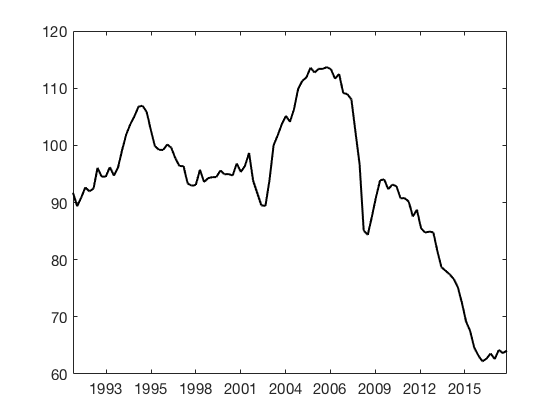
\includegraphics[width=\textwidth]{fig7}
        \caption{TCR}
    \end{subfigure}
    ~ %add desired spacing between images, e. g. ~, \quad, \qquad, \hfill etc. 
      %(or a blank line to force the subfigure onto a new line)
    \begin{subfigure}[b]{0.49\textwidth}
        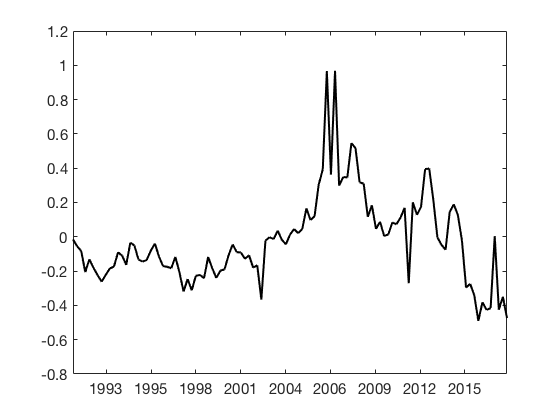
\includegraphics[width=\textwidth]{fig8}
        \caption{NFA}
    \end{subfigure}
    \begin{subfigure}[b]{0.49\textwidth}
        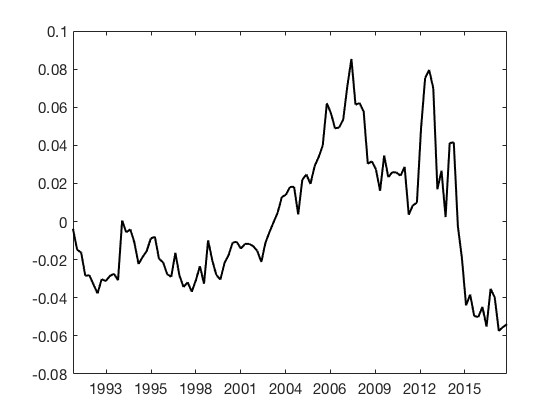
\includegraphics[width=\textwidth]{fig9}
        \caption{Saldo CC}
    \end{subfigure}
    ~ %add desired spacing between images, e. g. ~, \quad, \qquad, \hfill etc. 
    %(or a blank line to force the subfigure onto a new line)    
   \begin{subfigure}[b]{0.49\textwidth}
       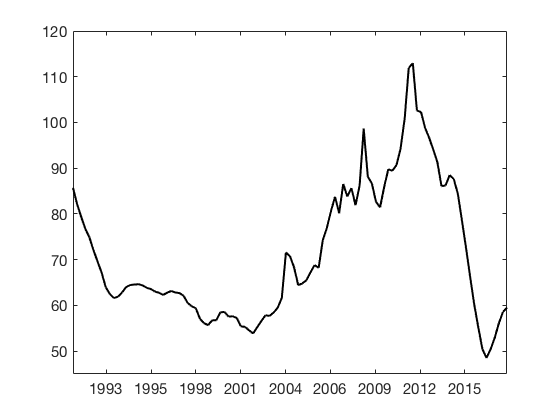
\includegraphics[width=\textwidth]{fig10}
        \caption{TI}
    \end{subfigure}
    \begin{subfigure}[b]{0.49\textwidth}
        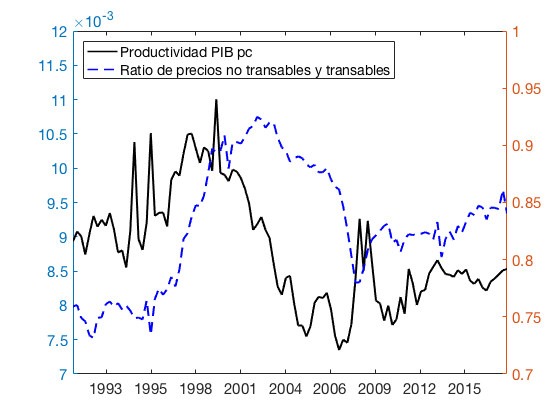
\includegraphics[width=\textwidth]{fig11}
        \caption{Productividad}
    \end{subfigure}
    ~ %add desired spacing between images, e. g. ~, \quad, \qquad, \hfill etc. 
      %(or a blank line to force the subfigure onto a new line)
    \begin{subfigure}[b]{0.49\textwidth}
        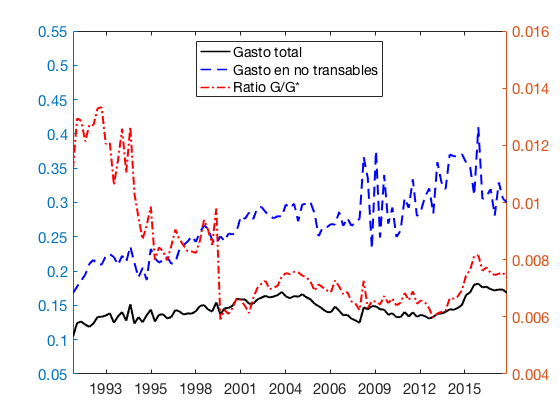
\includegraphics[width=\textwidth]{fig12}
        \caption{Gasto}
    \end{subfigure}
\end{figure}

\begin{table}
\caption{Matriz de correlación}
\begin{center}
\begin{tabular}{lcccccc}									
\hline													
\hline
							& 	\multicolumn{3}{c}{$TCR$}\\
							&	1991-2017	&	1991-2003	& 2004-2017	\\
\hline													
$PIBpc/PIBpc*$	&	-0,001		&	-0,477			&	-0,568			\\
$P_{NT}/P_T$		&	0,042		&	-0,609			&	0,395			\\
$G_{NT}/Y$			&	-0,498		&	-0,422			&	-0,559			\\
$GY^*/G^*Y$		&	0,102		&	-0,045			&	-0,197			\\
$G/Y$			 		&	-0,371		&	0,326			&	-0,443			\\
$P_X/P_M$			&	0,010		&	0,532			&	0,243			\\
$CC/Y$ 				&	0,467		&	0,587			&	0,705			\\
$AEN/Y$ 				&	0,414		&	0,832			&	0,704			\\
\hline													
\hline									
\end{tabular}	
\end{center}						
\begin{scriptsize}
\emph{Nota:} Elaboración propia.
\end{scriptsize}	
\label{correbeer}	
\end{table}	

La revisión de los gráficos delata un quiebre estructural en las relaciones de las variables con respecto al TCR, por lo tanto se contrasta en análisis gráfico con el soporte de correlaciones simples utilizando variables sin el componente estacional:
\begin{itemize}
\item Los términos de intercambio presentan una relación levemente procíclica aunque defasada. El cuadro \ref{correbeer} ratifica dicha prociclicidad aunque a un nivel bastante bajo, siendo que durante el primer periodo de corte se presenta la mayor correlación. Esto tiene sentido, debido a que la política cambiaria en dicho periodo estaba enfocada en utilizar las devaluaciones para mejorar el nivel del TCR para incentivar las exportaciones. Esta búsqueda de competitividad también estaba determinado por la presión que los términos de intercambio podrían haber generado, mayor devaluación para contrarestar el descenso de los términos de intercambio procurando la subida del TCR. Nótese que durante este periodo no se logró superávit en cuenta corriente a través de la balanza comercial a pesar de dicho esfuerzo.
\item Las medidas de gastos de gobierno tienen diferentes comportamientos. \emph{i)} El gasto no transable del gobierno presenta mucha estacionalidad y una relación contracíclica con relación al TCR, esta es la variable con mayor correlación con respecto a la variable dependiente. \emph{ii)} El gasto de gobierno como ratio al gasto de los socios comerciales de Bolivia no muestra una relación clara, las correlaciones son bastante bajas comparadas con las otras variables que sugiere contraciclidad. \emph{iii)} El gasto de gobierno total de Bolivia muestra mucha estacionalidad y parece tener una relación contracíclica con respecto al TCR, aunque previo al 2003 se ve cierta prociclidad.
\item  Las medidas de riqueza externa muestran una prociclidad con respecto al TCR, aunque parece que la medida $AEN/Y$ se adelanta al TCR mientras que $CC/Y$ reacciona al tipo de cambio real. Indudablemente, estas son las variables que comparten más correlación con la variable dependiente.
\end{itemize}



%\begin{figure}
%\captionsetup[subfigure]{aboveskip=-1pt,belowskip=-1pt}
%\centering
%\caption{Correlaciones}
%\captionsetup[subfigure]{font=scriptsize,labelfont=scriptsize}
%    \begin{subfigure}[b]{0.48\textwidth}
%        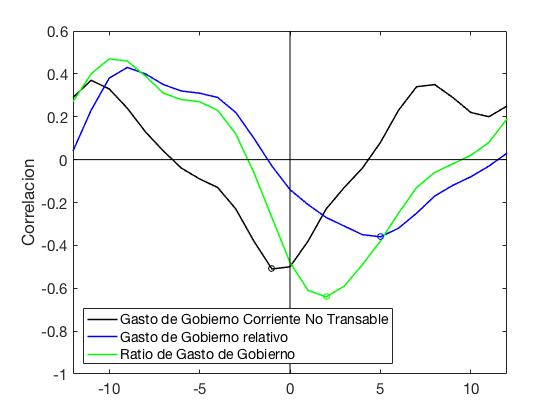
\includegraphics[width=\textwidth]{fig14}
%    \end{subfigure}
%    ~ %add desired spacing between images, e. g. ~, \quad, \qquad, \hfill etc. 
%      %(or a blank line to force the subfigure onto a new line)
%    \begin{subfigure}[b]{0.48\textwidth}
%        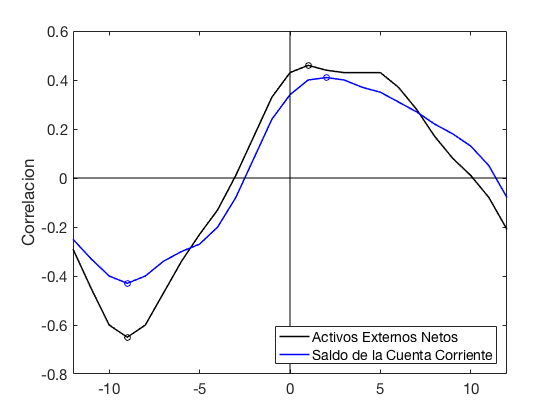
\includegraphics[width=\textwidth]{fig15}
%    \end{subfigure}
%    \begin{subfigure}[b]{0.48\textwidth}
%        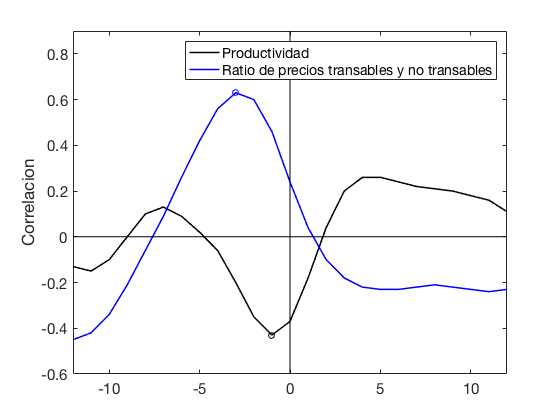
\includegraphics[width=\textwidth]{fig16}
%    \end{subfigure}
%    ~ %add desired spacing between images, e. g. ~, \quad, \qquad, \hfill etc. 
%    %(or a blank line to force the subfigure onto a new line)
%   \begin{subfigure}[b]{0.48\textwidth}
%       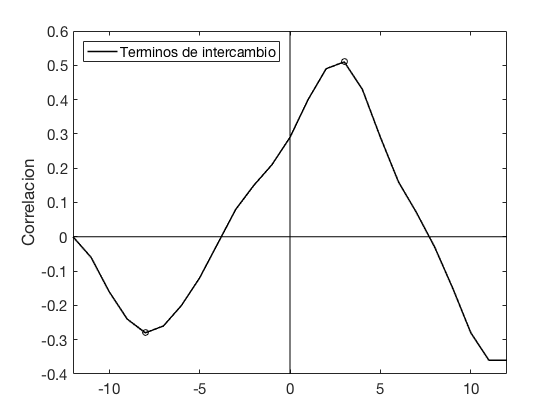
\includegraphics[width=\textwidth]{fig17}
%    \end{subfigure}  
%   \begin{subfigure}[b]{0.48\textwidth}
%       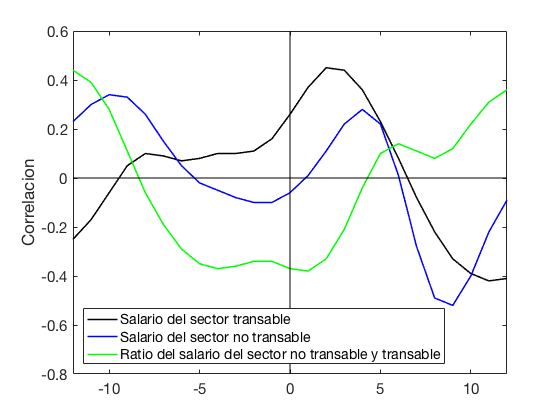
\includegraphics[width=\textwidth]{fig18}
%    \end{subfigure}
%\end{figure}

\begin{table}
\begin{center}
\caption{Modelos de cointegración, solo con intercepto en la relación de largo plazo}
\scalebox{0.8}{%
\begin{tabular}{lccccccc}
\hline
\hline
											&\multicolumn{2}{c}{(1)}&	(2)		&	(3)		&	(4)		&	(5)		\\
Variables							&	Vec 1	&	Vec 2	&			&			&			&			\\
\hline
											&	\multicolumn{6}{c}{Regresión de largo plazo}							\\
\hline													
$\ln (TCR)$						&	1					&1,338***		&	1				&	1				&	1				&	1		\\
											&						&	(0,055)		&					&					&					&			\\
$\ln (G/Y)$						&0,482***		&	1					&					&0,894***	&					&			\\
											&	(0,060)		&						&					&(0,205)		&					&			\\
$\ln (GY^*/G^*Y)$			&						&						&-0,220**	&					&-0,044		&			\\
											&						&						&	(0,088)	&					&(0,232)		&			\\
$\ln (G_{NT}/Y)$				&						&						&					&					&					&0,405***	\\
											&						&						&					&					&					&(0,158)	\\
$\ln (P_{NT}/P_T)$			&0,263***		&0						&					&					&0,336			&			\\
											&	(0,075)		&						&					&					&(0,748)		&			\\
$\ln (PIBpc/PIBpc*)$		&						&						&	0,253		&0,655***	&					&0,724**	\\
											&						&						&	(0,221)	&(0,235)		&					&(0,341)	\\
$\ln (P_X/P_M)$				&	0,553***		&0,794***		&0,409***	&0,748***	&0,610***	&0,632***	\\
											&	(0,098)		&(0,043)			&	(0,131)	&(0,139)		&(0,211)		&(0,167)	\\
$\ln (\tilde{CC}/Y)$		&-0,086**		&-0,131***		&-0,086**	&-0,091***	&					&			\\
											&	(0,033)		&	(0,043)		&(0,040)		&(0,030)		&					&			\\
$\ln (\tilde{AEN}/Y))$	&						&	 					&					&					&-0,280***	&-0,243***	\\
											&						&						&					&					&(0,034)		&(0,029)	\\
Constante							&	-6,163			&	-7,912			&	-6,405		&	-3,163		&-7,547		&-3,499		\\
\hline													
									&	\multicolumn{6}{c}{Velocidad de ajuste de cada variable}				\\
\hline													
$\Delta \ln (T	CR)$						&-0,269 		&	0,192			&	-0,053*	&	-0,020		&	0,017		&	0,019	\\
														&	(0,168)	&	(0,132)		&	(0,027)	&	(0,032)	&(0,014)		&(0,016)	\\
$\Delta \ln (G/Y)$						&1,128***	&-1,015***		&					&	-0,108*	&					&			\\
														&	(0,284)	&	(0,223)		&					&	(0,064)	&					&			\\
$\Delta\ln(GY^*/G^*Y)$				&					&						&	0,067		&					&	-0,056		&			\\
														&					&						&	(0,084)	&					&(0,044)		&			\\
$\Delta\ln(G_{NT}/Y)$				&					&						&					&					&					&-0,122**	\\
														&					&						&					&					&					&(0,055)	\\
$\Delta\ln(P_{NT}/P_T)$			&	-0,034*	&	0					&					&					&	-0,007		&			\\
														&(0,019)		&						&					&					&	(0,009)	&			\\
$\Delta\ln(PIBpc/PIBpc*)$		&					&						&	0,039		&	-0,024		&					&-0,008		\\
														&					&						&	(0,051)	&	(0,059)	&					&(0,030)	\\
$\Delta\ln(P_X/P_M)$					&-0,008		&-0,018			&	0,015		&	-0,053		&	0,004		&-0,015		\\
														&	(0,284)	&(0,223)			&	(0,046)	&	(0,051)	&(0,023)		&(0,027)	\\
$\Delta\ln(\tilde{CC}/Y)$		&21,894***	&-14,328***	&4,364***	&5,030***	&					&			\\
														&(5,135)		&	(4,025)		&	(0,843)	&	(0,989)	&					&			\\
$\Delta\ln(\tilde{AEN}/Y))$	&					&						&					&					&4,415***	&5,423***	\\
														&					&						&					&					&(0,712)		&(0,820)	\\
\hline													
\hline													
\end{tabular}%
}	
\end{center}
\begin{scriptsize}
\emph{Nota:} La significancia al uno, cinco y diez por ciento es indicada por ***, ** y *, respectivamente. Desviaciones estándar entre paréntesis. $\tilde{CC}/Y = \min CC/Y + \delta$ y $\tilde{AEN}/Y + \min AEN/Y + \delta $, donde $\delta \rightarrow 0$.
\end{scriptsize}						
\label{beercoi}		
\end{table}	

En el marco de la evidencia empírica descrita, se realiza la estimación de los modelos de cointragración. Los resultados resumen cinco especificaciones diferentes. La obtención de este reducido número de relaciones se logró probando las distintas opciones de variables proxys que se tiene a disposición para cumplir con la identificación propuesta previamente, se escogieron aquellas que representan la robustez de los resultados obtenidos.

Vale la pena recalcar que después de la remoción de los componentes estacionales bajo el método \emph{X-12 ARIMA}, se encontró una raíz unitaria estadística en todas las variables propuestas. La operativización de las variables se realizó a través de la transformación logarítimica como los resultados log-linealizados obtenidos por \cite{lane2004trans} y \cite{Obstfeld1995dynamics}. Posteriormente, se procedió a verificar la existencia de cointegración entre cada conjunto de variables utilizadas habiendo escogido los rezagos óptimos que permite la eliminación de autorrelación en los errores, mediante el método de Johansen. Se concluye que todos los modelos tienen una relación de cointegración mientras solo uno de ellos presentó dos vectores de cointegración.

El cuadro \ref{beercoi} muestra los resultados de las relaciones de largo plazo y los correspondientes parámetros de ajuste. Estos resultados corresponden a 5 relaciones más representativas. Para leer el cuadro, considérese que todas las variables en la regresión de largo plazo expuestas en el primer bloque del cuadro \ref{beercoi} deben igualar a cero, de forma que las variables independientes deben pasar al lado derecho con signo cambiado para obtener la representación convencional $\ln TCR_t=f(\ln Z_t)$. En general, se puede distinguir algunos resultados importantes:

Los términos de intercambio, los proxys de productividad y las representaciones de gasto público influyen en el largo plazo al TCR de manera negativa. La excepción radica en la variable de gasto público nacional respecto al gasto público del extranjero que es débilmente significativa y con influencia positiva. De estos tres conjuntos de variables los términos de intercambio son los más robustos y las representaciones de gasto las menos consistentes en significancia. Finalmente, ambas representaciones de riqueza externa tienen una influencia positiva en el TCR y son altamente robustas.

Con respecto a la velocidad de ajuste, las variables de riqueza externa reaccionan ajustándose positivamente a los cambios en el equilibrio de largo plazo rápidamente, mientras que el gasto, excluyendo la medida relativa con los socios comerciales, parecen ajustarse menos rápido y en dirección contraria a los desequilibrios en el corto plazo. En contraposición, las variables de productividad y términos de intercambio no se ajustan a los desequilibrios de corto plazo, además el TCR muestra relativa exogeneidad débil, con la excepción del expuesta en el segundo modelo que muestra una significancia al 10\%.

Los modelos de corrección de errores indican que las variables más significativas y robustas que influyen en el TCR son el mismo TCR y los activos externos netos generalmente en el primer rezago y los términos de intercambio de manera positiva dentro de los primeros dos rezagos. Por otro lado, las variables de corto plazo con menor robustez e influencia son las variables de gasto, productividad y cuenta corriente. Aquí se debe notar que a pesar que la cuenta corriente y los activos externos netos comparten la misma tendencia, los componentes cíclicos son diferentes y los de $AEN/Y$ tienen influencia en el TCR. Nótese que dentro las variables que afectan al TCR en el corto plazo, la principal variable sobre la cual la política económica podría tener cierto control es esta última.

A la luz de esta evidencia empírica se puede concluir que los modelos de cointegración dan testimonio de una relación fuerte de largo plazo del TCR especialmente con la riqueza externa y los términos de intercambio y en menor medida con el gasto y las medidas de productividad. Por otro lado, los gráficos \ref{grafbeer} y las correlaciones del cuadro \ref{correbeer} sugieren un quiebre de las relaciones de las variables alrededor de 2003. Esta sospecha motiva el corte de la muestra y reestimación de los modelos. Para tal efecto, los modelos pierden la robustez por la menor información contenida en ambas submuestras. Sin embargo, este ejercicio es significativo en el sentido que sugiere que una evaluación más profunda debe ser realizada. 

En este sentido, vale la pena aclarar que el objetivo de la presente sección es obtener el TCR de equilibrio para el periodo de tiempo con el que se cuentan datos (1991-2017) a través del método BEER. Para lo cual se emplean los primeros 3 modelos del cuadro \ref{beercoi} que se presentan en la figura \ref{beergraf}. Como ya había sido adelantado, el TCR se encuentra íntimamente relacionado con la tendencia de equilibrio calculada. Los fundamentos definen dicha trayectoria en todos los casos. Sin embargo, las variaciones de muy corto son determinadas por la riqueza externa y los términos de intercambio.

\begin{figure}
\centering
\caption{BEER}
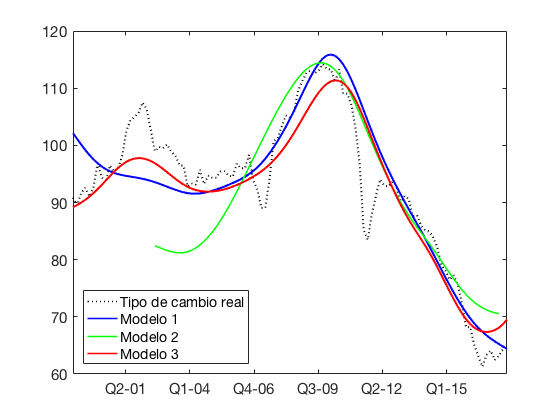
\includegraphics[scale=0.6]{fig19}
\label{beergraf}
\end{figure}

\subsection*{FEER}

%datos
El método se basa en estimar las elasticidades de comercio con respecto al TCR: $\eta_X$ y $\eta_M$, de las ecuaciones de exportaciones e importaciones reales \ref{X} y \ref{M}, respectivamente. Para lograr ese cometido, se verifican las propiedades individuales y en conjunto de las series en niveles. Nótese que todas las variables son integradas de grado 1 especialmente debido a la presencia de tendencias.

Las variables analizadas son: importación y exportación real (expresadas en moneda constante), PIB real de Bolivia (expresado en moneda constante), índice de los PIB de los principales socios comerciales de Bolivia, tipo de cambio real e índice de precios exportados por Bolivia. Mientras que el PIB, importaciones y exportaciones de Bolivia son de fuente Instituto Nacional de Estadística de Bolivia (INE)\footnote{Más adelante se utiliza los datos de la cuenta corriente boliviana, la misma que es fuente BCB. Hubiese sido ideal trabajar con las series de exportación e importación de la balanza de pagos del BCB pues estas son las series utilizadas para calcular la cuenta corriente. Sin embargo, el cambio de metodología (al Manual de Balanza de Pagos 6, MBP6) bajo el cual se tienen calculados unicamente los años 2014, 2015 y 2016, hace imposible la concatenación de datos con los años pasados que están calculados bajo otras metodologías, por esta razón se opta por utilizar los respectivos datos con fuente del INE.}, las restantes variables son creadas y mantenidas por el \emph{BCB} (Banco Central de Bolivia). Todas las variables han sido desestacionalizadas por el métodos \emph{X-12 ARIMA}.

\begin{figure}
\centering
%\captionsetup[subfigure]{aboveskip=-2pt,belowskip=-2pt}
\caption{Variables incluidas en el modelo}\label{variables}
    \begin{subfigure}[b]{0.4\textwidth}
        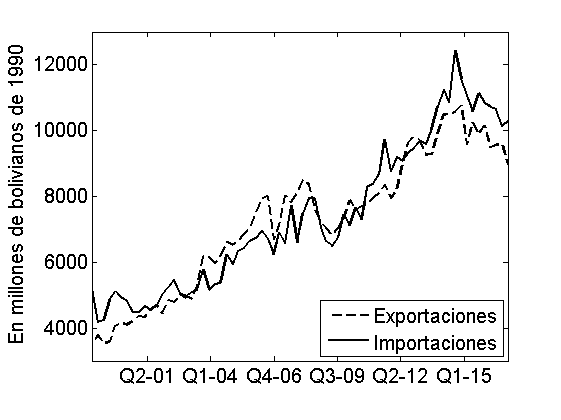
\includegraphics[width=\textwidth]{1xm}
        \caption{Exportación e importación}
        \label{1xm}
    \end{subfigure}
    ~ %add desired spacing between images, e. g. ~, \quad, \qquad, \hfill etc. 
      %(or a blank line to force the subfigure onto a new line)
    \begin{subfigure}[b]{0.4\textwidth}
        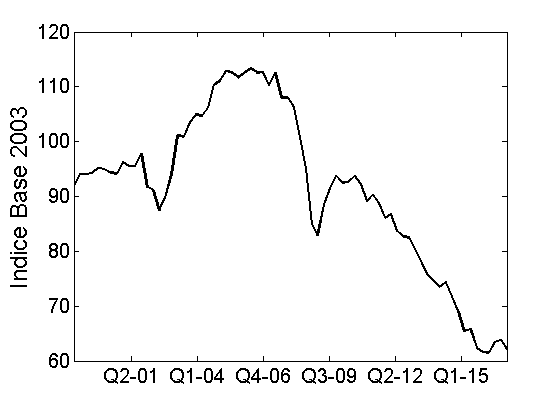
\includegraphics[width=\textwidth]{3tcr}
        \caption{TCR}
        \label{3tcr}
    \end{subfigure}
    \begin{subfigure}[b]{0.4\textwidth}
        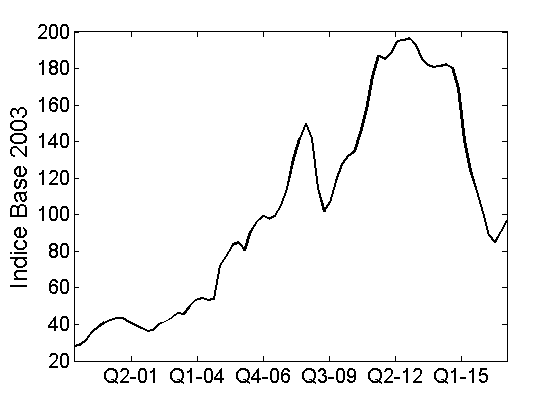
\includegraphics[width=\textwidth]{5ippbx}
        \caption{Precios internacionales}
        \label{5ippbx}
    \end{subfigure}
    ~ %add desired spacing between images, e. g. ~, \quad, \qquad, \hfill etc. 
      %(or a blank line to force the subfigure onto a new line)
    \begin{subfigure}[b]{0.4\textwidth}
        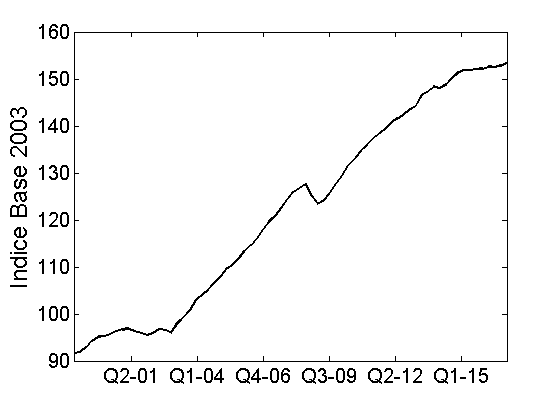
\includegraphics[width=\textwidth]{2per}
        \caption{PIB externo relevante}
        \label{2per}
    \end{subfigure}
    \begin{subfigure}[b]{0.4\textwidth}
        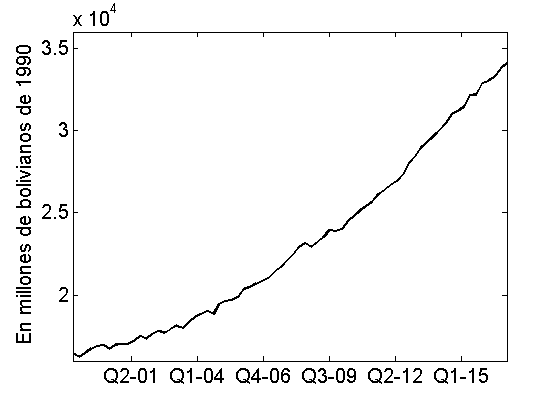
\includegraphics[width=\textwidth]{4pib}
        \caption{PIB}
        \label{4pib}
    \end{subfigure}
\end{figure}

En principio, la verificación gráfica sugiere que las series de importación y exportación comparten tendencia con el PIB de Bolivia y el índice de producto de sus principales socios comerciales, respectivamente. En el comportamiento del PIB boliviano se advierte una tendencia de crecimiento sostenido desde 1999, sin embargo, desde aproximadamente el 2009, esta presenta una aceleración que dura hasta 2013. El índice del PIB de los socios comerciales más importantes de Bolivia muestra una recesión en 2008 marcada por la crisis financiera internacional y un desaceleramiento a partir de 2013. Esta última variable parece reflejar mejor la tendencia del comercio internacional boliviano al compartir tendencia con las exportaciones. A pesar de que la serie del tipo de cambio real no parece presentar una relación en tendencia tan evidente como la señalada previamente, el índice de precios de productos bolivianos exportados parece compartir ciclos con la serie de exportaciones.

\begin{table}
\caption{Matriz de correlación}
\begin{center}
\begin{tabular}{lcccccc}									
\hline													
\hline												
	&	Exportaciones	&	Importaciones	&	PIB externo	&	TCR	&	IPPBX	&	PIB	\\
\hline													
Exportaciones	&	1	&		&		&		&		&		\\
Importaciones	&	0.9384	&	1	&		&		&		&		\\
PIB externo	&	0.9424	&	0.9751	&	1	&		&		&		\\
TCR	&	-0.5185	&	-0.7131	&	-0.7103	&	1	&		&		\\
IPPBX	&	0.8949	&	0.8506	&	0.8743	&	-0.3589	&	1	&		\\
PIB	&	0.9017	&	0.9645	&	0.9835	&	-0.8102	&	0.7821	&	1	\\
\hline													
\hline									
\end{tabular}	
\end{center}						
\begin{scriptsize}
\emph{Nota:} Elaboración propia.
\end{scriptsize}	
\label{corre}	
\end{table}	

Para verificar el análisis gráfico se calcula la matriz de correlación de las variables previamente señaladas, las cuales se muestran en la tabla \ref{corre}. Como había sido adelantado, el PIB externo relevante es la variable más fuertemente asociada a las exportaciones e importaciones seguidas por PIB boliviano y el índice de precios de exportaciones que, como era de esperar, está más correlacionado con las exportaciones. Por otro lado, el tipo de cambio real presenta una correlación negativa con ambas variables especialmente con las importaciones. Bajo este adelanto parece ser que los signos propuestos en la ecuación \ref{M} se cumplirían mientras que en la ecuación \ref{X} el TCR presentaría el signo contrario al esperado.

\begin{table}
\caption{Regresiones de Comercio Naïve}
\begin{center}
\scalebox{0.8}{%
\begin{tabular}{lcccc}									
\hline									
\hline	
						&	(1)				&	(2)			&	(3)			&	(4)	\\
						&	$x$			&	$\Delta x$	& $m$			&	$\Delta m$	\\
\hline	
$y^*$				&	1,670***	&					&					&		\\
						&	(0,024)		&					&					&		\\
$\Delta y^*$		&					&	1,369**		&					&		\\
						&					&	(0,585)		&					&		\\
$y$					&					&					&	1,060***	&		\\
						&					&					&	(0,018)		&		\\
$\Delta y$			&					&					&					&	1,088**		\\
						&					&					&					&	(0,479)	\\
$tcr$				&	0,072***	&					&	-0,384***	&	\\
						&	(0,023)		&					&	(0,035)		&	\\
$\Delta tcr$		&					&	0,362*		&					&	-0,174	\\
						&					&	(0,195)		&					&	(0,235)	\\
\hline									
\hline									
\end{tabular}%
}
\end{center}
\begin{scriptsize}
\emph{Nota:} La significancia al uno, cinco y diez por ciento es indicada por ***, ** y *, respectivamente. Desviaciones estándar entre paréntesis.
\end{scriptsize}								
\label{Rec}	
\end{table}	

En el cuadro \ref{Rec} se resume los resultados de las regresiones de comercio en las que las correspondientes variables se encuentran logaritmizadas y fueron identificadas en las ecuaciones \ref{X} y \ref{M}. Asimismo, se recalca que al haber establecido una identificación específica para el cálculo de DEER se respetará dicha identificación a través del estudio concluyendo la pertinencia de la misma en el caso boliviano. Se ensayan dos regresiones lineares primero en niveles y después en diferencias. Los resultados en niveles representan las relaciones de largo plazo por entenderse que las series de comercio comparten tendencia con sus correspondientes demandas, sin considerarse explícitamente su relación cointegrante. Por otro lado, los resultados en diferencias corresponden a las relaciones de corto plazo y están asociadas a la relación de los componentes cíclicos de las series.

En primer lugar, se debe aclarar que el cuadro \ref{Rec} evidencia que las relaciones de largo plazo son mucho más significativas y presentan los signos esperados. Efectivamente, este resultado se desprende del hecho que las series comparten tendencias y están cointegradas. Los resultados muestran elasticidad en las exportaciones y elasticidad unitaria en las importaciones con respecto a sus demandas, estos resultados se repiten en el corto plazo aunque con menor significancia. Asimismo, la relación de largo plazo de las exportaciones es más inelástica que la de las importaciones con respecto al TCR.

En el corto plazo, las variaciones alrededor de la tendencia del TCR no tienen efecto en las importaciones, mientras que las exportaciones muestran inelasticidad significativa aunque relativamente moderada. La baja significancia genera la sospecha que, especialmente en las importaciones, existen otros componentes como términos de intercambio y precios que podrían ayudar a determinar mejor las variaciones a corto plazo de las series de comercio. Sin embargo, se debe entender que si se consideran al TCR como un precio relativo, el efecto ingreso domina la dinámica que determina el comercio exterior.

Como ya ha sido adelantado, el cuadro \ref{Rec} está compuesto por regresiones que ignoran la relación de cointegración de las variables en cuestión. En vista de la integración de grado 1 de todas las variables se procede con las pruebas de cointegración con el número de rezagos apropiados el modelo de corrección de errores. Se encuentra que ambas relaciones presentan un solo vector de cointegración. Los resultados de los modelos estimados son presentados en los cuadros \ref{cointx} y \ref{cointm}.

\begin{table}
\caption{Cointegración en la Exportación }
\begin{center}
\scalebox{0.8}{%
\begin{tabular}{lccccccccc}									
\hline									
\hline
							&	\multicolumn{3}{c}{(1)}								&	\multicolumn{3}{c}{(2)}								&	\multicolumn{3}{c}{(3)}								\\
							&	$x$			&						&						&	$x$			&						&						&	$x$			&						&						\\
\hline
$y^*$					&	1,640***	&						&						&	1,548***	&						&						&	1,603***	&						&						\\
							& (0,094)		&						&						& (0,101)		&						&						& (0,117)		&						&						\\	
$tcr$					& 0,030		&						&						& 0,174**		&						&						& 0,130			&						&						\\
							& (0,091)		&						&						& (0,097)		&						&						& (0,113)		&						&						\\
\hline
							& $\Delta x$	&	$\Delta y^*$	&	$\Delta tcr$	& $\Delta x$	&	$\Delta y^*$	&	$\Delta tcr$	& $\Delta x$	&	$\Delta y^*$	&	$\Delta tcr$	\\
$\alpha$				& -0,022		& 0,016***		& -0,012			& -0,141***	& 	0					& -0,054**		& -0,139**	& 	0					& 0					\\
							& (0,031)		& (0,003)			& (0,015)			& (0,060)		& 	Restr			& (0,029)			& (0,066)		& 	Restr			& Restr				\\
\hline
$\Delta x_{-1}$		& -0,279***	& -0,003			& 0,038			& -0,219**	& -0,003			& 0,057			& -0,201**	& -0,000			& 0,058			\\
							& (0,101)		& (0,009)			& (0,049)			& (0,103)		& (0,011)			& (0,051)			& (0,105)		& (0,011)			& (0,052)			\\
$\Delta x_{-2}$		& -0,199**	& -0,003			& -0,011			& -0,156*		& -0,002			& 0,002			& -0,145*		& 0,000			& 0,002			\\
							& (0,098)		& (0,009) 			& (0,048)			& (0,098)		& (0,010) 			& (0,048)			& (0,099)		& (0,011) 			& (0,049)			\\
$\Delta y^*_{-1}$	& 2,750***	& 0,401***		& 0,699*			& 2,750***	& 0,599***		& 0,643*			& 2,524***	& 0,635***		& 0,557*			\\
							& (0,999)		& (0,094)			&	(0,487)			& (0,884)		& (0,093)			&	(0,436)			& (0,869)		& (0,094)			&	(0,430)			\\
$\Delta y^*_{-2}$	& 0,165			& -0,060			& -0,790**		& 0,230		& 0,089			& -0,811**			& 0,099		& 0,118				& -0,869**		\\
							& (0,984)		& (0,092) 			& (0,480)			& (0,910)		& (0,096) 			& (0,449)			& (0,898)		& (0,097) 			& (0,445)			\\
$\Delta tcr_{-1}$	& 0,004		& 0,039**			& 0,205**			& -0,055		& 0,035**			& 0,187**			& -0,042		& 0,030*			& 0,195**			\\
							& (0,204)		& (0,019)			& (0,099)			& (0,202)		& (0,021)			& (0,099)			& (0,200)		& (0,022)			& (0,099)			\\
$\Delta tcr_{-2}$	& 0,193			& 0,049***		&-0,091			& 0,129			& 0,034*			&-0,107			& 0,158			& 0,026			&-0,093			\\
							& (0,206)		& (0,019)			& (0,101)			& (0,201)		& (0,021)			& (0,099)			& (0,198)		& (0,021)			& (0,098)			\\
\hline									
\hline
\end{tabular}%
}
\end{center}
\begin{scriptsize}
\emph{Nota:} La significancia al uno, cinco y diez por ciento es indicada por ***, ** y *, respectivamente. Desviaciones estándar entre paréntesis.
\end{scriptsize}								
\label{cointx}	
\end{table}	

Los resultados de largo plazo de la relación de exportaciones expuestos en el cuadro \ref{cointx} confirman una relación de elasticidad elevada y significativa del volumen comerciado con respecto a la demanda externa. A diferencia de los modelos \emph{naïve}, la elasticidad precio, es decir la correspondiente al TCR, es no significativa y cercana a cero en las regresiones (1) y (3). La relación de corto plazo del modelo de corrección de errores muestra inelasticidad no significativa del TCR con respecto a las exportaciones. A este último resultado, se suma la exogeneidad débil que presenta el TCR en la ecuación (1). Estos resultados confirman que no hay relación de tendencias entre el volumen de exportaciones y el TCR, mientras que los componentes cíclicos de corto plazo de estas variables están disociados. Entonces, ante los desequilibrios de la relación de largo plazo estudiada, el TCR no realiza ningún tipo de ajuste para restablecer dicho equilibrio. En contraposición, la demanda externa tiene gran influencia y es bastante elástica tanto en el largo como el corto plazo. En las regresiones (2) y (3) se ensayan dos restricciones. En (2) se plantea la nulidad del coeficiente de ajuste de largo plazo para la demanda externa, esto debido a que esta no se ajusta a los desequilibrios de la relación de largo plazo de exportaciones bolivianas debido al tamaño de la economía boliviana y la participación minoritaria que tiene en las importaciones totales de sus socios comerciales. La regresión (3) impone exogeneidad débil para la demanda externa y el TCR, lo cual tiene sentido desde la perspectiva de los resultados encontrados en la regresión (1) y porque el desajuste de la relación de largo plazo de las exportaciones no es realizado a través del TCR. En otras palabras, esto quiere decir que la identificación planteada determina a las exportaciones como la variable endógena y a la demanda externa y el TCR como variables exógenas. La imposición de restricciones de exogeneidad débil en el contexto de cointegración permite acercarse a esta identificación manteniendo la coherencia del comportamiento económico de las series.

Sin embargo, a pesar de la importancia de que la demanda externa y el TCR sean exógenamente débiles, las pruebas chi cuadrado descartan el planteamiento de los modelos restringidos. Esto es importante para la interpretación del modelo y la conclusión que se pueda obtener del mismo. Como ya se ha mencionado, el tamaño de la economía boliviana y el flujo comercial de Bolivia a sus socios comerciales hace que el crecimiento económico extranjero sea altamente independiente de las exportaciones bolivianas. Mientras que por lo contrario, las exportaciones bolivianas dependan altamente de la demanda externa que está determinada por el crecimiento económico de los socios comerciales de Bolivia. Al mismo tiempo, si bien después de 1985 hasta 2005 se ancló la política cambiaria a un comportamiento de depreciación sostenida con el objetivo de obtener superávits comerciales, el periodo posterior a 2005 se caracterizó por desenlazar este objetivo con el instrumento de la política cambiaria, siendo que esta última se concentró en utilizar la apreciación como complemento - parte central en realidad - de la política monetaria para apaciguar presiones de inflación importada y mantener las expectativas de tipo de cambio de la población. El resultado del primer periodo de depreciación, marcado por fallar en lograr la meta de superávits con la política cambiaria descrita, y el rol monetario del segundo periodo implican que el TCR sea efectivamente débilmente exógeno. En este sentido, el rechazo estadístico a dichas restricciones corresponde a la potencial mala o incompleta identificación de estos modelos de exportación. De esto depende la evaluación del modelo DEER examinado más adelante.

\begin{table}
\caption{Cointegración en la Importación}
\begin{center}
\scalebox{0.8}{%
\begin{tabular}{lccc}									
\hline									
\hline	
							&	\multicolumn{3}{c}{(1)}									&	\multicolumn{3}{c}{(2)}								&
							&	$m$				&						&						&	$m$				&						&						\\
\hline			
$y$						&	0,729***		&						&						&	0,818***		&						&						\\
							& (0,161)			&						&						& (0,107)			&						&						\\	
$tcr$					& -0,059			&						&						& -0,118			&						&						\\
							& (0,304)			&						&						& (0,202)			&						&						\\	
\hline
							& $\Delta m$	&	$\Delta y$		&	$\Delta tcr$	& $\Delta m$	&	$\Delta y$		&	$\Delta tcr$	\\
$\alpha$				& -0,032***		& 0,010***		&	0,007			& -0,050***		& 0,015***		& 0					\\
							& (0,013)			& (0,002)			& (0,006)			& (0,020)			& (0,003)			& Restr				\\
\hline
$\Delta m_{-1}$		& -0,397***		& -0,004			& 0,018				& -0,386***		& -0,008			& 0,014				\\
							& (0,098)			& (0,015)			& (0,044)			& (0,097)			& (0,015)			& (0,043)			\\
$\Delta m_{-2}$	& -0,200**		& -0,009			& -0,022			& -0,191**			& -0,013			& -0,026			\\
							& (0,099)			& (0,015)			& (0,044)			& (0,097)			& (0,015)			& (0,044)			\\
$\Delta m_{-3}$	& -0,350***		& -0.001			& -0,038			& -0,342***		& -0.003			& -0,041			\\
							& (0,097)			& (0,015)			& (0,043)			& (0,097)			& (0,015)			& (0,043)			\\
$\Delta m_{-4}$	& -0,272***		& -0,029**		& -0,023			& -0,268***		& -0,030**		& -0,025			\\
							& (0,094)			& (0,014)			& (0,042)			& (0,093)			& (0,014)			& (0,042)			\\
$\Delta y_{-1}$		& 1,695***		& -0,279***		& -0,531**		& 1,697***		& -0,266***		& -0,480*			\\
							& (0,686)			& (-2,725)			& (0,305)			& (0,677)			& (-0,102)			& (0,303)			\\
$\Delta y_{-2}$		& 2,863***		& -0,032			& -0,541**		& 2,873***		& -0,016			& -0,468*			\\
							& (0,748)			& (0,112)			& (0,332)			& (0,736)			& (0,111)			& (0,329)			\\
$\Delta y_{-3}$		& 2,498***		& 0,028			& -0,250			& 2,515***		& 0,044			& -0,172			\\
							& (0,796)			& (0,119)			& (0,354)			& (0,784)			& (0,118)			& (0,351)			\\
$\Delta y_{-4}$		& -0,272***		& -0,029**		& -0,023			& 0,535			& -0,067			& 0,109				\\
							& (0,094)			& (0,014)			& (0,042)			& (0,699)			& (0,105)			& (0,313)			\\
$\Delta tcr_{-1}$	& 0,494**			& -0,015			& 0,209**			& 0,483**			& -0,011			& 0,214**			\\
							& (0,231)			& (0,034)			& (0,102)			& (0,230)			& (0,035)			& (0,103)			\\
$\Delta tcr_{-2}$	& -0,015			& -0,023			& -0,084			& -0,019			& -0,021			& -0,079			\\
							& (0,243)			& (0,036)			& (0,108)			& (0,242)			& (0,036)			& (0,108)			\\
$\Delta tcr_{-3}$	& 0,041				& -0,013			& 0,035			& 0,035			& -0,011			& 0,038			\\
							& (0,237)			& (0,035)			& (0,106)			& (0,237)			& (0,036)			& (0,106)			\\
$\Delta tcr_{-4}$	& 0,388**			& 0,035			& -0,002			& 0,377**			& 0,038			& -0,002			\\
							& (0,229)			& (0,034)			& (0,102)			& (0,229)			& (0,034)			& (0,102)			\\
\hline									
\hline									
\end{tabular}%
}
\end{center}
\begin{scriptsize}
\emph{Nota:} La significancia al uno, cinco y diez por ciento es indicada por ***, ** y *, respectivamente. Desviaciones estándar entre paréntesis.
\end{scriptsize}								
\label{cointm}	
\end{table}	

El modelo de cointegración de las importaciones presentado en el cuadro \ref{cointm} muestra resultados similares a los planteados para el caso de las exportaciones. Comparando los cuadros \ref{Rec} y \ref{cointm} para el caso de las importaciones se verifica que la cointegración corrige la relación de largo plazo planteando una sensibilidad baja y no significativa con respecto al TCR. Por otro lado, en el corto plazo el TCR parece afectar a las importaciones aunque no con el signo esperado. Además, se confirma la exogeneidad débil del TCR, mientras que el ingreso y las propias importaciones son las que corrigen los desequilibrios de la relación de largo plazo. La regresión (2) determina un modelo restringido que no es rechazado por los tests estadísticos siendo, entonces, el mejor modelo especificado. Finalmente, se nota que existe una relación significativa pero inelástica en el largo plazo de las importaciones con respecto a la demanda interna. Sin embargo, en el corto plazo existe una relación altamente significativa y elástica con esta última variable. Se debe notar que a diferencia de las regresiones de exportación, no se puede entender a la demanda interna caracterizada por el PIB como débilmente exógena pues desde el lado del gasto esta variable depende directamente de ella. La significancia de la inelasticidad del TCR en el corto plazo implica un signo preocupante de la dinámica particular que sucede en la economía boliviana que será discutida más adelante.

En suma, esto implica que el comercio internacional está definido en el largo y corto plazo por la demanda tanto interna como externa. La debilidad de los modelos de exportación se debe a que parece existir otro tipo de idiosincracias constituidas por los costos de producción locales, costos de exportación, competitividad del volumen relativo a otras ofertas internacionales que cubran determinada demanda, costos de transporte, tratados comerciales y calidad de la producción que no fueron tomados en cuenta en esta identificación. Sin embargo, los resultados de estos modelos implican que la consideración competitiva de los volúmenes de exportaciones sean exógenos a los impactos de política monetaria y cambiaria que puedan ser propuestos principalmente porque el TCR que caracteriza a estas políticas no tiene relación con el tipo de exportaciones bolivianas como se discutirá en el próximo párrafo. Por otro lado, las importaciones dependen del ingreso que la población tenga en la economía. Este efecto ingreso sobrepasa el efecto precio ajustado por tipo de cambio sugiriendo la falta de posibilidad de sustituir estas importaciones con respecto a la producción nacional, esta es la razón por la que los parámetros estimados de corto y largo plazo del cuadro \ref{cointm} no sean significativos, incluso ante shocks de depreciación del TCR las importaciones crecen por la incapacidad de sustituirlos internamente por lo que se obtienen parámetros estimados con signos sospechosamente cambiados.

\begin{figure}
\captionsetup[subfigure]{aboveskip=-2pt,belowskip=-2pt}
\centering
\caption{Estructura de importaciones y exportaciones de Bolivia}\label{impexp}
    \begin{subfigure}[h]{0.65\textwidth}
        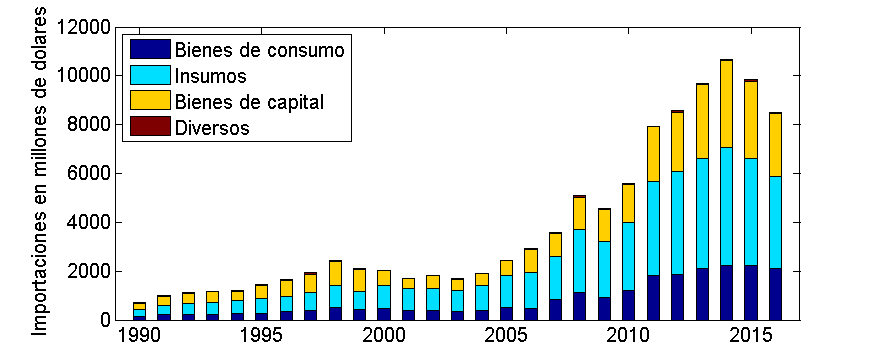
\includegraphics[width=\textwidth]{imp9016}
        \caption{Estructura de importaciones}
        \label{mestr}
    \end{subfigure}
    \begin{subfigure}[h]{0.65\textwidth}
        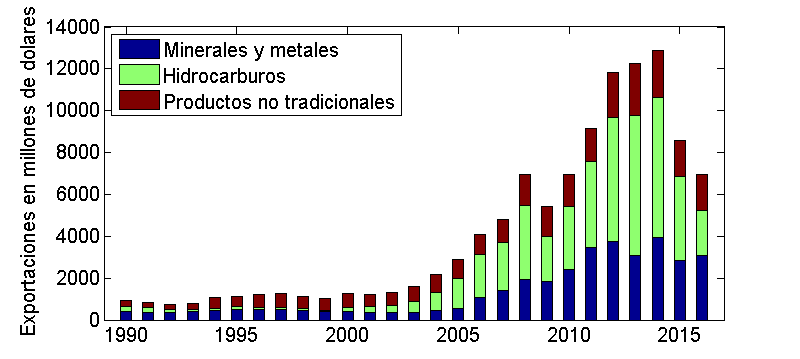
\includegraphics[width=\textwidth]{exp9016}
        \caption{Estructura de exportaciones}
        \label{xestr}
    \end{subfigure}
\end{figure}

En este sentido, nótese en el gráfico \ref{3tcr} que el TCR se aprecia sostenidamente entre 2007-2016.\footnote{Obviando el quiebre que sucedió durante la crisis financiera internacional que al final no afecto a la tendencia del comportamiento del TCR.} Este comportamiento, contrastado con la figura \ref{impexp}, coincide con el crecimiento sustancial de las exportaciones e importaciones. Mientras la teoría indica que una apreciación de estas características debería haber afectado negativamente a las exportaciones y positivamente a las importaciones, la evidencia muestra que dicha apreciación favoreció de manera positiva a ambas series.

La explicación de este fenómeno depende de las características particulares de lo que sucedió en ese periodo. Las exportaciones bolivianas de hidrocarburos y minerales representan, en promedio, el 78\% desde el incremento de los precios internacionales de materias primas en 2004 y alcanzan los niveles más elevados de participación entre 2011-2014. El producto que lidera el incremento de las exportaciones es el gas cuyo boom en ventas se vio favorecido por el ciclo de precios elevados de materias primas suscitado desde 2004 y 2005 que coincide con la firma de contratos de exportación con Brasil y Argentina, lo cual asegura la venta de este producto a estos mercados que a su vez se vieron favorecidos internamente por el incremento de precios de materias primas que incrementó sus ingresos gracias al comercio internacional, determinando así el crecimiento sostenido de la demanda externa para Bolivia para su principal producto de exportación. Es necesario recalcar que todas las exportaciones se vieron favorecidas por el incremento de la demanda externa mundial de materias primas, bienes intermedios y finales. El fin de esta parte del ciclo de grandes volúmenes de exportación se materializa en Bolivia después de 2014 con la caída de los precios de exportación que recién en el 2016 y 2017 comienzan a recuperarse.

En este sentido se debe entender como es que se mide el TCR para comprender la disociación establecida en los modelos que existe entre estas variables. El tipo de cambio real no mide los precios de las materias primas, recuérdese que para calcular este indicador se utiliza los índices de precios al consumidor, el cual toma en cuenta productos de una canasta de consumo, es decir bienes finales de consumo cotidiano por el consumidor representativo y no así productos primarios e intermedios cuya demanda la componen productores. A priori se estima que por construcción esta variable solo tendría una influencia con la exportación de bienes finales y manufacturas, las cuales se encuentran dentro de la categoría de no tradicionales de la figura \ref{impexp} pero representan una parte muy pequeña de estas. Las manufacturas oscilan en participación entre 12-25\% entre 1999-2006 y 7-12\% en 2007-2016 siendo este último periodo en el que el volumen exportado de manufacturas se llegó a multiplicar por lo menos por tres mostrando un crecimiento muy significativo a pesar de la apreciación del TCR. Esto explica la disociación de corto plazo y la insignificancia de largo plazo del TCR en las exportaciones.

Por el lado de las importaciones, la estructura no es tan variable a través de los años a pesar del incremento notable suscitado en 2004 y confirmado en 2005. La pregunta es: porqué la marcada correlación positiva de crecimiento y apreciación no generaron elasticidades positivas de TCR en los modelos del cuadro \ref{Rec}. La respuesta yace en el hecho que prima el efecto ingreso en dichas realizaciones, eso quiere decir que sin importar el encarecimiento relativo de los bienes extranjeros, el incremento del ingreso nacional impulsó la demanda de importaciones fuertemente. Es por este motivo que se registra una alta elasticidad con respecto a la demanda caracterizada por el PIB local. Además, nótese que Bolivia importa una gran cantidad de insumos y bienes de capital que no son representados por el TCR. 

La baja sensibilidad del comercio al tipo de cambio real implica que sea necesario cambios muy elevados de este para generar variaciones significativas en el comercio externo boliviano, aunque estos podrían ser insostenibles o incluso perjudiciales para otros sectores de la economía.

Haciendo uso de las elasticidades de las ecuaciones 1 y 3 de la tabla \ref{Rec} se construye la serie estimada del TCR de equilibrio con operativizando la ecuación \ref{qfeer}. Posteriormente se estima la varianza de la ecuación citada. Los resultados son mostrados y contrastados con las series de cuenta corriente observada y objetivo y el correspondiente desalineamiento de TCR con respecto a la serie obsevada en la figura \ref{deerq}.

\begin{figure}
%\captionsetup[subfigure]{aboveskip=-2pt,belowskip=-2pt}
\caption{Resultados DEER}
\centering
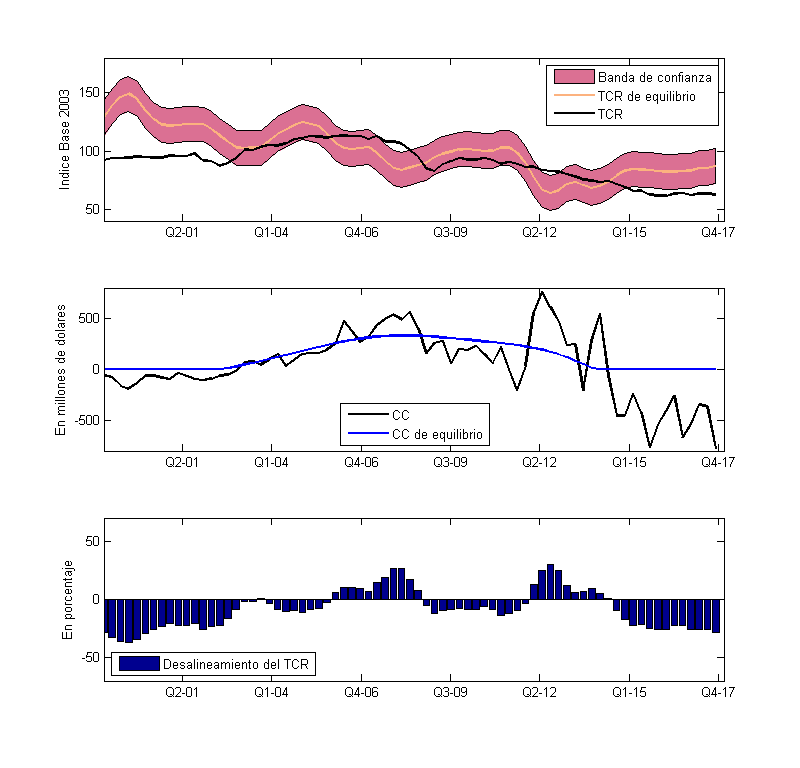
\includegraphics[scale=0.7]{tcreq}
\label{deerq}
\end{figure}

De esta evidencia se verifica que el tipo de cambio real estuvo desalineado de forma importante durante dos periodos de la muestra planteada 2000-2006 y 2014-2017. A partir del 2006 la diferencia entre el tipo de cambio real observado y de equilibrio tiende a ser mucho menor. A partir del 2014 la divergencia de ambas series comienza a ser fuerte. En estos periodos de desequilibrio se entiende que el tipo de cambio real se encontraba sobre-valuado. Es decir que para restaurar el equilibrio era necesario fomentar la devaluación del TCR. En efecto, si verificamos paralelamente a los tipos de cambio reales observados y de equilibrio junto con la cuenta corriente observada y de objetivo podemos verificar que los desalineamientos en tipo de cambio coinciden con los de cuenta corriente. 

Por otro lado, durante los periodos 2004-2005 y 2009-2011, la devaluación del TCR podría haber sido beneficiosa para sostener los niveles de superávit alcanzados para minimizar las variaciones significativas de la cuenta corriente en dichos periodos.

Desde esta óptica, es importante verificar que la mayor variación de cuenta corriente correspondiente a 2013 con una tendencia pronunciada al déficit ya eran indicios importantes para gestionar la política adecuada de depreciación del tipo de cambio real para poder conseguir el equilibrio externo y evitar los déficits incurridos posteriormente.

Es importante notar que las variaciones de tipo de cambio son un tema particularmente delicado en Bolivia por la historia inflacionaria y el hecho que la economía está anclada nominalmente al valor del dólar. Por otro lado, al ser las exportaciones dependientes del precio de las materias primas que comercia internacionalmente un buen indicador de la dirección que la balanza comercial, y por ende, la cuenta corriente vayan a tomar son los precios de materias primas exportadas.

Otro punto interesante de estos resultados se enfoca en el periodo previo a 2006. El mismo implica que durante esta época el tipo de cambio real no estuvo alineado con sus valores de equilibrio pues la cuenta corriente se hallaba en un estado deficitario. Esto a pesar de que la constante depreciación del tipo de cambio nominal estaba determinada por valor referencial objetivo que supuestamente indica la depreciación nominal necesaria para mantener el tipo de cambio real constante y competitivo. Evidentemente, esta política cambiaria no funcionó, por lo menos no para incentivar los superávit de cuenta corriente y balanza comercial.

%\footnote{Si bien esto es cierto, en la realidad los bienes primarios transados bilateralmente entre países tienen como precio aplicable aquel pactado en los contratos suscritos entre partes, el cual puede ser o no el mismo que los determinados por los mercados internacionales, tal vez debido a otros factores como la calidad o el costo de transporte u otras consideraciones. Sin embargo, y sin lugar a dudas estos precios internacionales son el referente de los precios últimos contratados por materias primas.}	

\section{Consideraciones Preliminares}\label{consid}

%\subsection*{Movimientos del tipo de cambio real}
Debido a que la fórmula de tipo de cambio real es la definida por \ref{tcr1} o \ref{tcrlog} y el tipo de cambio nominal es el principal instrumento de la política cambiaria, se hace tentador simplemente despejar esta variable de la fórmula para que ella indique cual, para el nivel deseado de tipo de cambio real, es el nivel de depreciación nominal necesario para lograr el nivel de TCR definido. Este es el método mediante el cual se encuentra el tipo de cambio referencial al que se hace mención previamente. Sin embargo, el uso de esta estrategia puede ser considerado una falacia teórica.

La razón es porque, en contraposición de los precios extranjeros que son exógenos, los precios de la economía doméstica dependen, o están en función entre otras cosas, del tipo de cambio nominal $p(e)$ que directamente determina el precio en moneda local de las importaciones nacionales. Al respecto, la evidencia más grande está en la literatura de \emph{pass-through} de tipo de cambio a inflación, la cuál generalmente obtiene valores significativamente distintos de cero y positivos. El hecho que el coeficiente de \emph{pass-through} sea distinto de cero implica que la depreciación del tipo de cambio nominal, desde una perspectiva de instrumento, genera presiones en el nivel de precios hacia el alza. Entonces, tanto el tipo de cambio nominal como el nivel de precios se incrementan determinando que en el corto plazo el efecto de una devaluación nominal se aminore en el ámbito del TCR a través de las importaciones que efectivamente determinan parte del índice de precios al consumidor.

En la realidad existen dos factores empíricos importantes que matizan esta situación. El efecto \emph{pass-through} no se da inmediatamente debido a la rigidez de precios, es decir que la transmisión del incremento del tipo de cambio a los precios no ocurre inmediatamente sino a medida que los precios se reajustan a dicho cambio, únicamente una economía con total flexibilidad de precios o indexada perfectamente a la divisa de referencia transmitiría inmediatamente dicho efecto. Por otro lado, es un caso muy extremo cuando el parámetro \emph{pass-through} llegue a ser unitario pues implicaría que no solamente el sector transable es perfectamente sensible sino también el sector no transable lo es, en cuyo caso se podría pensar que el tipo de cambio afecta a los costos importados de bienes no transables. Otra probable explicación es que el efecto en los precios transables y no transables sobre-reaccionen debido a las expectativas inflacionarias y/o devaluativas haciendo que el efecto total de \emph{pass-through} llegue a la unidad, lo cual implicaría que la economía se encuentra en una posición demasiado riesgosa.

Otra consideración importante es que el nivel de \emph{pass-through} es variable, es decir que no es fijo a través del tiempo y depende de la situación particular en el que cada economía esté. Esto probablemente debido a la formación de las expectativas de los agentes. Por tanto, el uso adecuado del tipo de cambio nominal es complicado y sensible a varias consideraciones.

En el caso de Bolivia, el uso de la regla cambiaria siguiendo el tipo de cambio de referecia, previamente mencionado, no logró el efecto esperado en el comercio internacional. Durante el periodo en el que esta política de determinación de las devaluaciones estuvo vigente (2005), el tipo de cambio real se situó volátilmente bajo su meta la cual puede ser caracterizada como 100 en el gráfico \ref{3tcr}.

En realidad, lo que demuestra el comportamiento durante 1990 y 2003 es que la velocidad de la depreciación es menor que el de los precios internos dado el ajuste al nivel de precios externos exógenos. Potencialmente, esto implicaría que la aceleración de la depreciación generaría una velocidad aún mayor en el nivel de precios local. Esto implica que no se logra tomar en cuenta el efecto inflacionario de la devaluación en el nivel de precios locales. En particular, el desajuste de TCR entre 1994 y 1995 se debe principalmente al repunte inflacionario de Brasil, uno de los principales socios comerciales de Bolivia, que en estas fechas introduce el real como moneda oficial, este factor externo originó que la moneda boliviana se deprecie más de lo esperado en términos reales. Al mismo tiempo, este evento se constituye en un shock que marca la leve desaceleración de la depreciación boliviana que no es tan pronunciada como la sugerida por su tipo de cambio referencial.

Es posible que la moderada depreciación y el anclaje de la expectativas de los agentes en la misma depreciación colaboró a que la inflación importada de Bolivia no sea incluso más elevada. Sin embargo, este hecho demuestra empíricamente la falacia teórica acerca de como mover el tipo de cambio real haciendo uso de su contraparte nominal.

\section*{Conclusiones}\label{concl}

Los modelos muestran que bajo el objetivo de sostenibilidad externa, los mayores desajustes corresponden a los periodos en los que la cuenta corriente se encuentra en desequilibrio principalmente por los déficits en balanza comercial. Al mismo tiempo, estos periodos coinciden con aquellos en los que los precios de materias primas no fueron lo suficientemente beneficiosos para el esquema comercial internacional boliviano.

A pesar de que hasta 2004 se siguió una regla cambiaria que buscaba determinar al tipo de cambio real en un nivel fijo de competitividad, la evidencia muestra que esta política falló fuertemente, pues no consideró que al depreciar el tipo de cambio nominal, este se contrarrestaría con el movimiento de la inflación importada determinada por el efecto \emph{pass-through}, este es sólo uno de los motivos por los que esta regla cambiaria no funcionó para conservar un nivel estable de tipo de cambio real, Rodrik menciona otro, la falta de capacidad para generar ilusión monetaria. Al mismo tiempo, las mini-devaluaciones solamente sirvieron para ayudar un pequeño grupo de exportadores de manufacturas, mientras que hacía que las importaciones se encarecieran constantemente en términos de la moneda boliviana, esta es la raiz de una sostenida inflación importada y de la dolarización de ese periodo debido a que las expectativas cambiarias de la población estaban ancladas en la depreciación.

A su vez, estos efectos en la economía boliviana podrían haber generado un marcado crecimiento de la participación de bienes finales de productores foráneos con mayor productividad en los mercados locales. Siendo que la demanda local se refugiaba en el dólar para poder acceder a la compra de bienes importados que se encarecían por la depreciación sostenida, la importación optó por el contrabando para poder vender productos más baratos. En este punto se debe considerar el bajo poder adquisitivo de la población que no lograba acceder a niveles de ingreso suficientes y accedían al mercado de bienes contrabandeados.

Durante el boom de los precios de materias primas y muy en especial después de la nacionalización de hidrocarburos en Bolivia el 2006 se vivió la recuperación de la balanza comercial. Este hecho representó una gran entrada de divisas a la economía que fortaleció a las RIN y dotó de suficientes dólares para cubrir los requerimientos del mercado interno. La apreciación real de la moneda significó que en este periodo de auge económico sea conveniente importar bienes dada el alza de ingresos y dicha apreciación fomentando el sector del comercio. Por otro lado, el ancla nominal cambiaria se fijó en la estabilidad del boliviano que contribuyó a la des-dolarización financiera de la economía.

Finalmente, después de la caída de precios internacionales de materias primas, la economía boliviana logró sobrevivir por la solidez ganada en periodos previos y los aún significativos ingresos de hidrocarburos. Sin embargo, la cuenta corriente se vio afectada así como las RIN en aras de sostener el ingreso interno de la población para poder fomentar la demanda interna. Si bien durante este periodo la opinión pública reclamó una depreciación nominal, se considera que, por la evidencia expuesta previamente, esta medida no podría haber podido cumplir el fin deseado de nivelar de nuevo la balanza comercial debido a que el volumen de la exportación de gas y minerales no dependen de esta variable y quizás dicha devaluación podría haber causado efectos negativos en otras áreas de la economía.

Como se ha visto, la estabilidad cambiaria es un gran aporte para la des-dolarización de la economía, sin embargo, el gobierno boliviano no ha encontrado aún la manera de mantener un tipo de cambio real estable y la evidencia señala que aún está experimentando con los instrumentos que tiene a su disposición. Asimismo, el auge económico respaldado por el comercio internacional fue patrocinado por el incremento de los precios del gas que también coincidió con la apreciación del tipo de cambio real y la débil consecución de la regla cambiaria que posteriormente fue abandonada al encontrar en en la estabilidad un refugio para permitir que la moneda local se fortalezca en el mercado interno que fue beneficiado por bajos precios de importaciones que a su vez beneficiaron a la mayor parte de la población que se dedica a este rubro y que a su vez permitió el crecimiento del sector no transable del país.

%La regla cambiaria utilizada es incorrecta porque no determina la dirección del TCR, este punto ya ha sido probado hace tiempo.

%Bolivia necesita entre otras cosas una industria que produzca transables y no transables sustituibles dentro de la economía y fuera también, sin eso estamos dependiendo fuertemente de los designios de los movimientos de la economía extranjera.

En esa línea, la segunda metodología permitió establecer los fundamentos que se asocian al tipo de cambio real de equilibrio, los más consistentes fueron el gasto de gobierno, los términos de intercambio, los activos externos netos y la productividad de transables con respecto a no transables. Este análisis permitió identificar que según la evidencia empírica por lo general los fundamentos tienden a anticipar los movimientos del tipo de cambio real, en esa línea el gasto de gobierno y las medidas de productividad mantienen la relación que se espera, mientras que los términos de intercambio transmitirían un efecto riqueza y no uno de sustitución. Si bien según la metodología se espera que el valor del tipo de cambio real se mantenga alineado se constan quiebres específicos, asociados a factores internos y externos, en los que se observan desalineamientos, sin embargo según esta metodología el TCR se mantiene en línea con la evolución de sus fundamentos. 

%Posibilidad de enfermedad holandesa. no existe porque no hay otro sector que se pueda matar.


%Hay que entender que el tipo de cambio real está calculado en base a las variaciones de los índices de precios al consumidor de los socios comerciales y local y de los tipos de cambio. Como se toma en cuenta los índices de precios al consumidor, esta medida captura la variación real de artículos que entran en la canasta básica de consumo de cada país. Es evidente que esta puede diferir entre economías, sin embargo, el cálculo del tipo de cambio real hace abstracción de estas divergencias y asume que son lo suficientemente parecidas. El punto importante que se debe notar es que captura los precios de bienes de consumo interno y que están dentro de la canasta básica, los cuales no son bienes que Bolivia exporta, en contraposición si son bienes que importa. Por este motivo es que la inclusión de los valores 


\bibliographystyle{apalike}
\bibliography{tcr_bolivia}
\end{document}
